\section{Reward network from healthy samples} \label{s:N_II:rwd}

\vspace{3mm}
% \noindent\rule{17cm}{0.2pt}
\fbox {
    \parbox{\linewidth}{
      \begin{itemize}
        \item 14 highly connected communities
        \item 122 genes with high mutation burden and a high number of strong correlations
        \item Healthy dataset and network pipeline reveals lncRNA genes to have an important role in MIBC subtyping
      \end{itemize}
    }
}
\vspace{3mm}

% Introducing the reward
The reward network is constructed following the pipeline in \cref{s:N_II:methods} where the sigmoid modifier is used to reward the mutated genes and iMEV takes in account the expression in both tumour and non-tumours data. Compared to the standard network, the correlations (or nodes' weights) of the mutated genes are increased proportionally with the mutation burden from TCGA's MIBC cohort. As in the previous section, the network is constructed from the same 5000 most varied genes from non-tumour dataset (see \cref{s:N_II:methods}) which compromises of ABS-Ca, P0 and UD samples.

% Describe the network 
% - small and large communities
The output networm is shown in \cref{fig:N_II:reward_net} where it can be observed that there  is a large variation in the community sizes. On the left hand side there is a group of small communities, while on the other side there are larger blocks of nodes such as community 0 (blue) or purple (9) at top. The community size imbalance was evident from the network metrics the comparison in \cref{fig:N_II:net_metric_sig_std}, which suggested that the reward network contains nodes that are highly connected.

% Talk about the aspects of the networks
Overexpression and dysregulation of the \textit{AHR} gene promotes tumour formation and it is present the Luminal samples \citep{Shi2020-km}. In \cref{fig:N_II:reward_net}, the red-lines are the edges from the \textit{AHR} gene/node to its neighbours gene which are mostly situated in the largest community (0).  It was also observed that it is usually the case that smaller communities have genes with a high degree and most of the edges lead to the larger communities. The genes in the large blocks (e.g., 0 or 9) are not connected with each other but these nodes seems to be grouped by their links to the genes in the smaller communities; like community \textbf{2} of which \textit{AHR} is part of. The small and highly connected communities are explored in more depth in the following sections.

% Size imbalance 

\begin{figure}[H]    
    \centering
    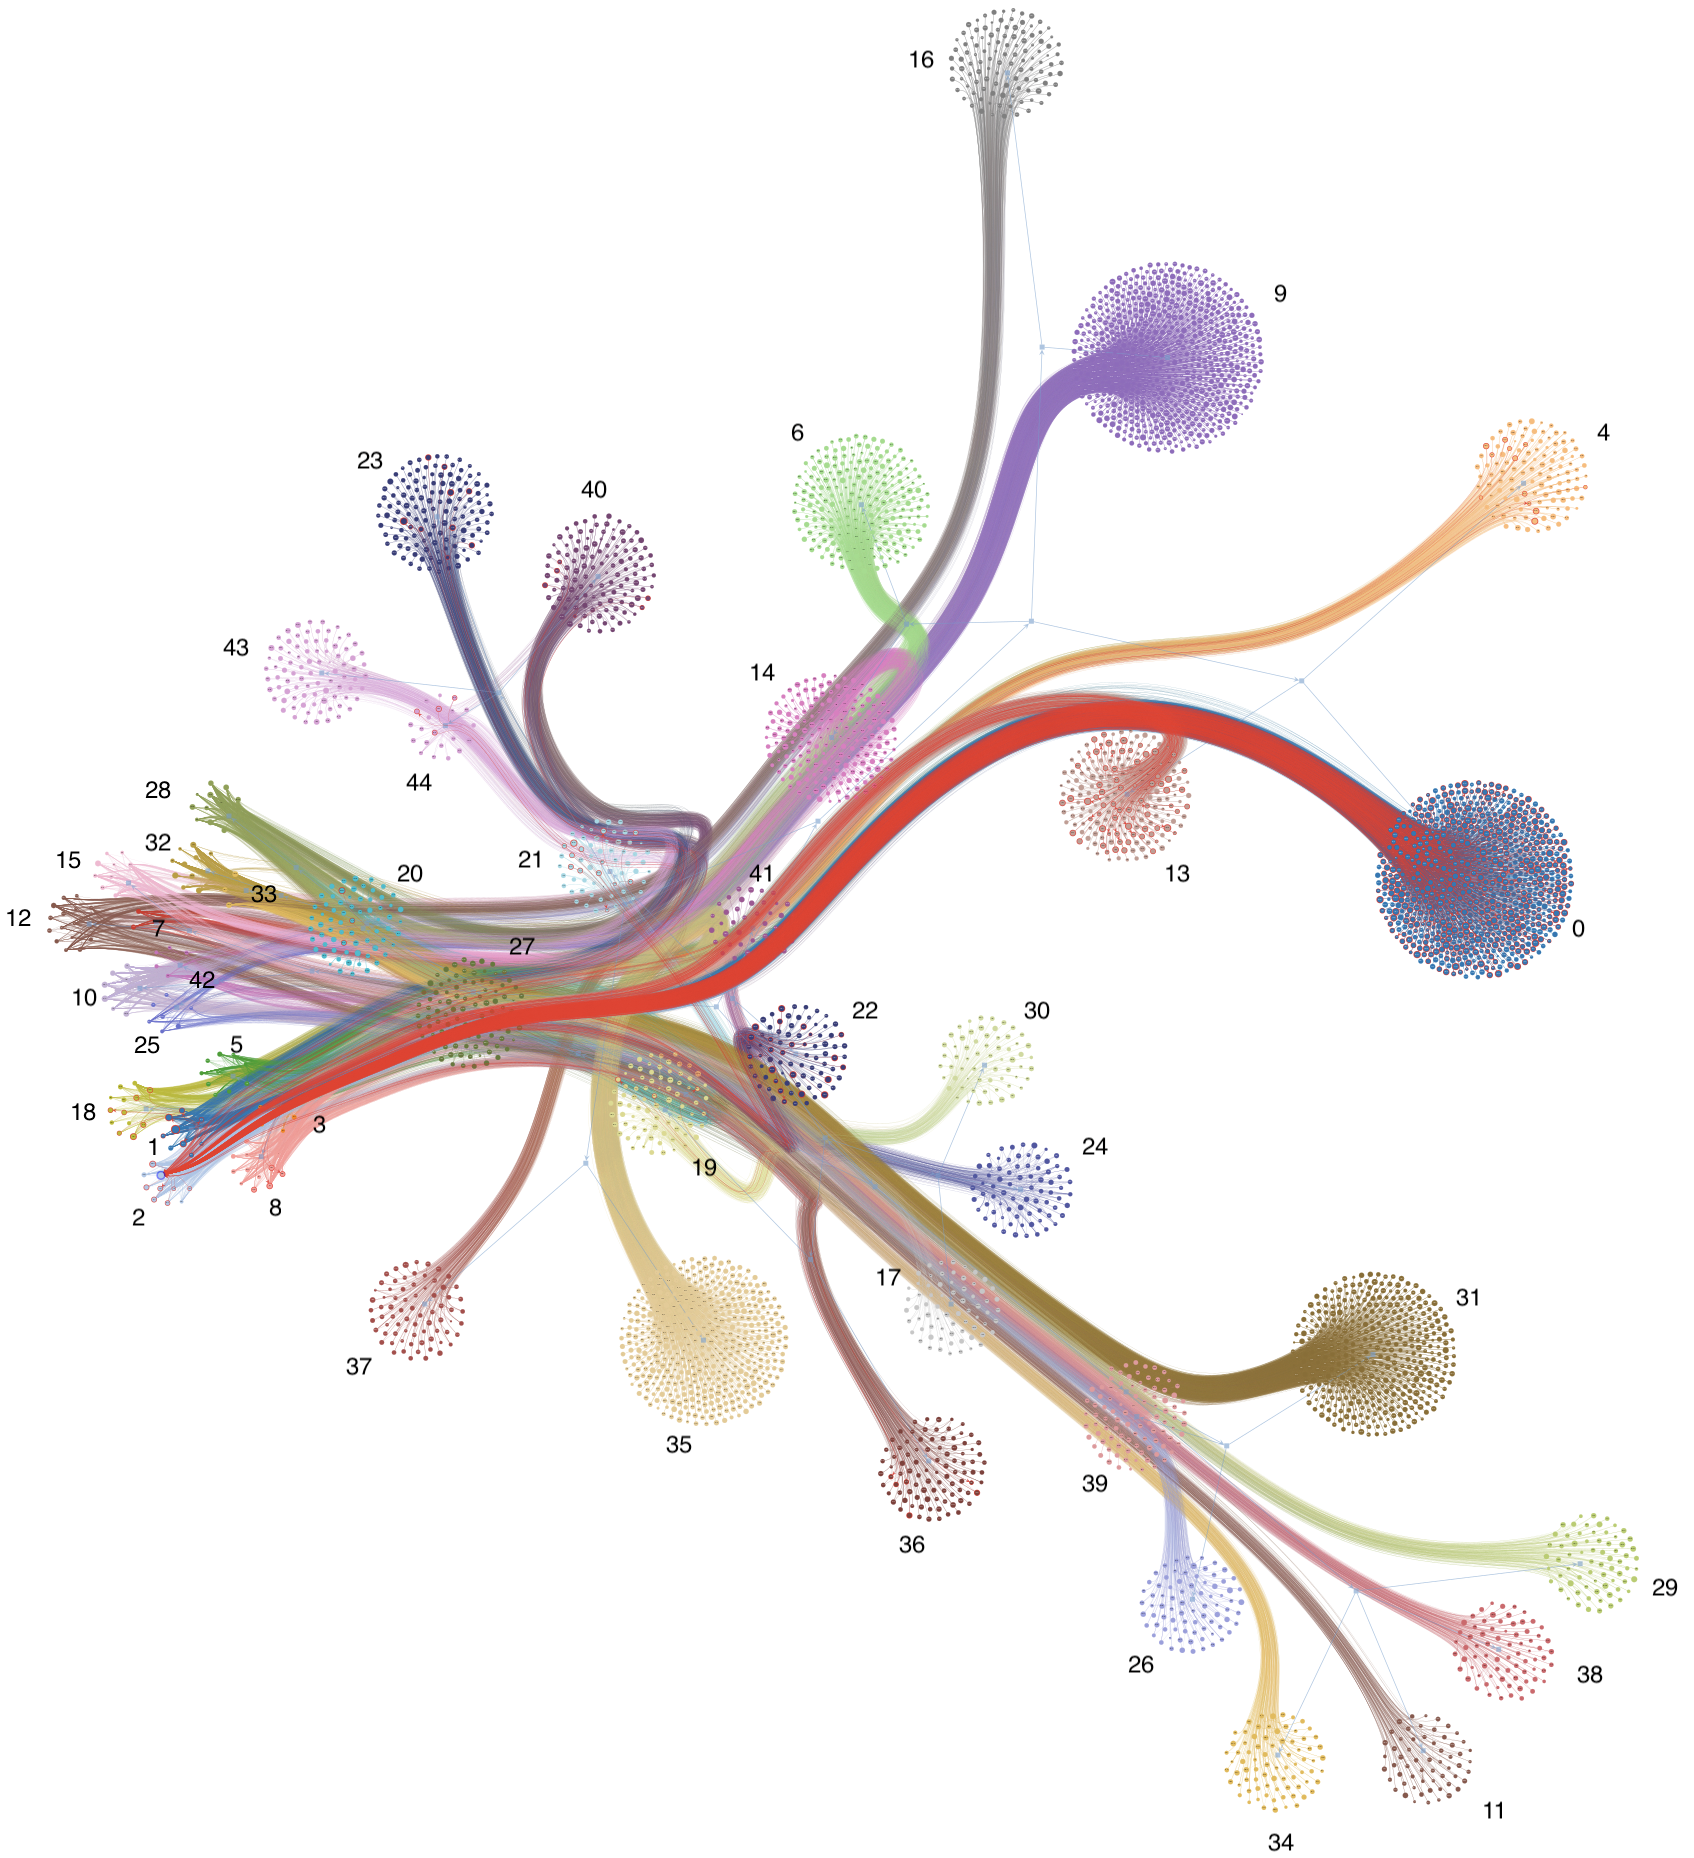
\includegraphics[width=1.0\textwidth,height=1.0\textheight,keepaspectratio]{Sections/Network_II/resources/reward/sigmoid_5K_Net_II_label_2.png}
    \caption[Reward network from healthy dataset with mutation burden]{The reward network constructed from the 5000 most relatively varied genes, 3 edges per standard and 6 for TF, hierarchical SBM is used for community detection. The connections in red represents the the edges between \textit{AHR} and other genes, showing the importance of the gene in the network. It can also be noticed that there are are some very small communities (e.g. 10, 8, 7) compared to very large groups of nodes such as 0 or 35. One striking aspect of the network is the community size imbalance, there are a few groups of genes with $<$10 nodes (e.g. 1, 2, 7) and others with a few hundreds (e.g., 0 or 9).}
    \label{fig:N_II:reward_net}
\end{figure}


% Highly connected genes
\subsection{High degree genes} \label{s:N_II:high_conn}

% Present the figure
To further understand the relationship between the size of a community (Y-axis) and the nodes' degree (mean values on the X-axis), the two properties were plotted on a scatter plot in \cref{fig:N_II:largeSmall_com}. The marker sizes in the figure are proportional to their mean mutation burden; the larger the point, the the mpre the gene is mutated across MIBC cohort. A community is labelled as "HighDegree" when the mean degree of the genes constituting the groups is in the 70th percentile, and as "LowDegree" otherwise. The 70th percentile was chosen as the threshold because it includes all the small communities.

% Talk about the community size imbalance
The positioning of communities with highly connected genes near the X-axis and those with less connected genes near the Y-axis indicates an inverse relationship between group size and degree. The analysis of the network metrics in \cref{fig:N_II:net_metrics_comp} highlighted a subset of nodes with high degree and lower closeness scores. However, it was unexpected that the hSBM would be able to isolate these nodes into separate groups to such an extent. Previously, a subset of highly connected nodes was observed in different network analyses, but the impact of the reward modifiers (v1 or v2) was not as pronounced as in this case. Specifically:
\begin{itemize}
    \item All graphs generated from the freshly isolated samples contained a subset of highly connected genes, more so than the tumour-generated networks, but this was not significantly amplified by the reward modifier (v1) - see network metrics in \cref{fig:N_I:net_metrics_p0}.
    \item Networks generated from the tumour dataset using the initial network approach from \cref{s:N_I:methods_edge_pruning} also exhibited a subset of highly connected nodes - see network metrics in \cref{fig:N_I:net_metrics_tum}.
    \item In the tumour networks analysed in this chapter, the reward modifier (v2) does not amplify the number of connections to the same extent as in the healthy graps - see network metrics in \cref{fig:N_II:net_metrics_comp}.
\end{itemize}

% High correlation
The inverse relationship between node degree and the community size as well as the effect of the reward modifier (v2)  is further confirmed by the negative Spearman correlation of $\rho = -0.8987$ and $p = 5.46$x$10^{-17}$; see \cref{fig:N_II:genes_highConn}, The positive correlation between community size and the average mutation count in a group indicates that well-connected communities have a high mutation burden. The multi-plot in Appendix \cref{fig:ap:degree_com_size} provides a clearer depiction of the mean degree and group size of the communities in the reward network, complementing \cref{fig:N_II:largeSmall_com}.

\begin{figure}[!b]    
    \centering
    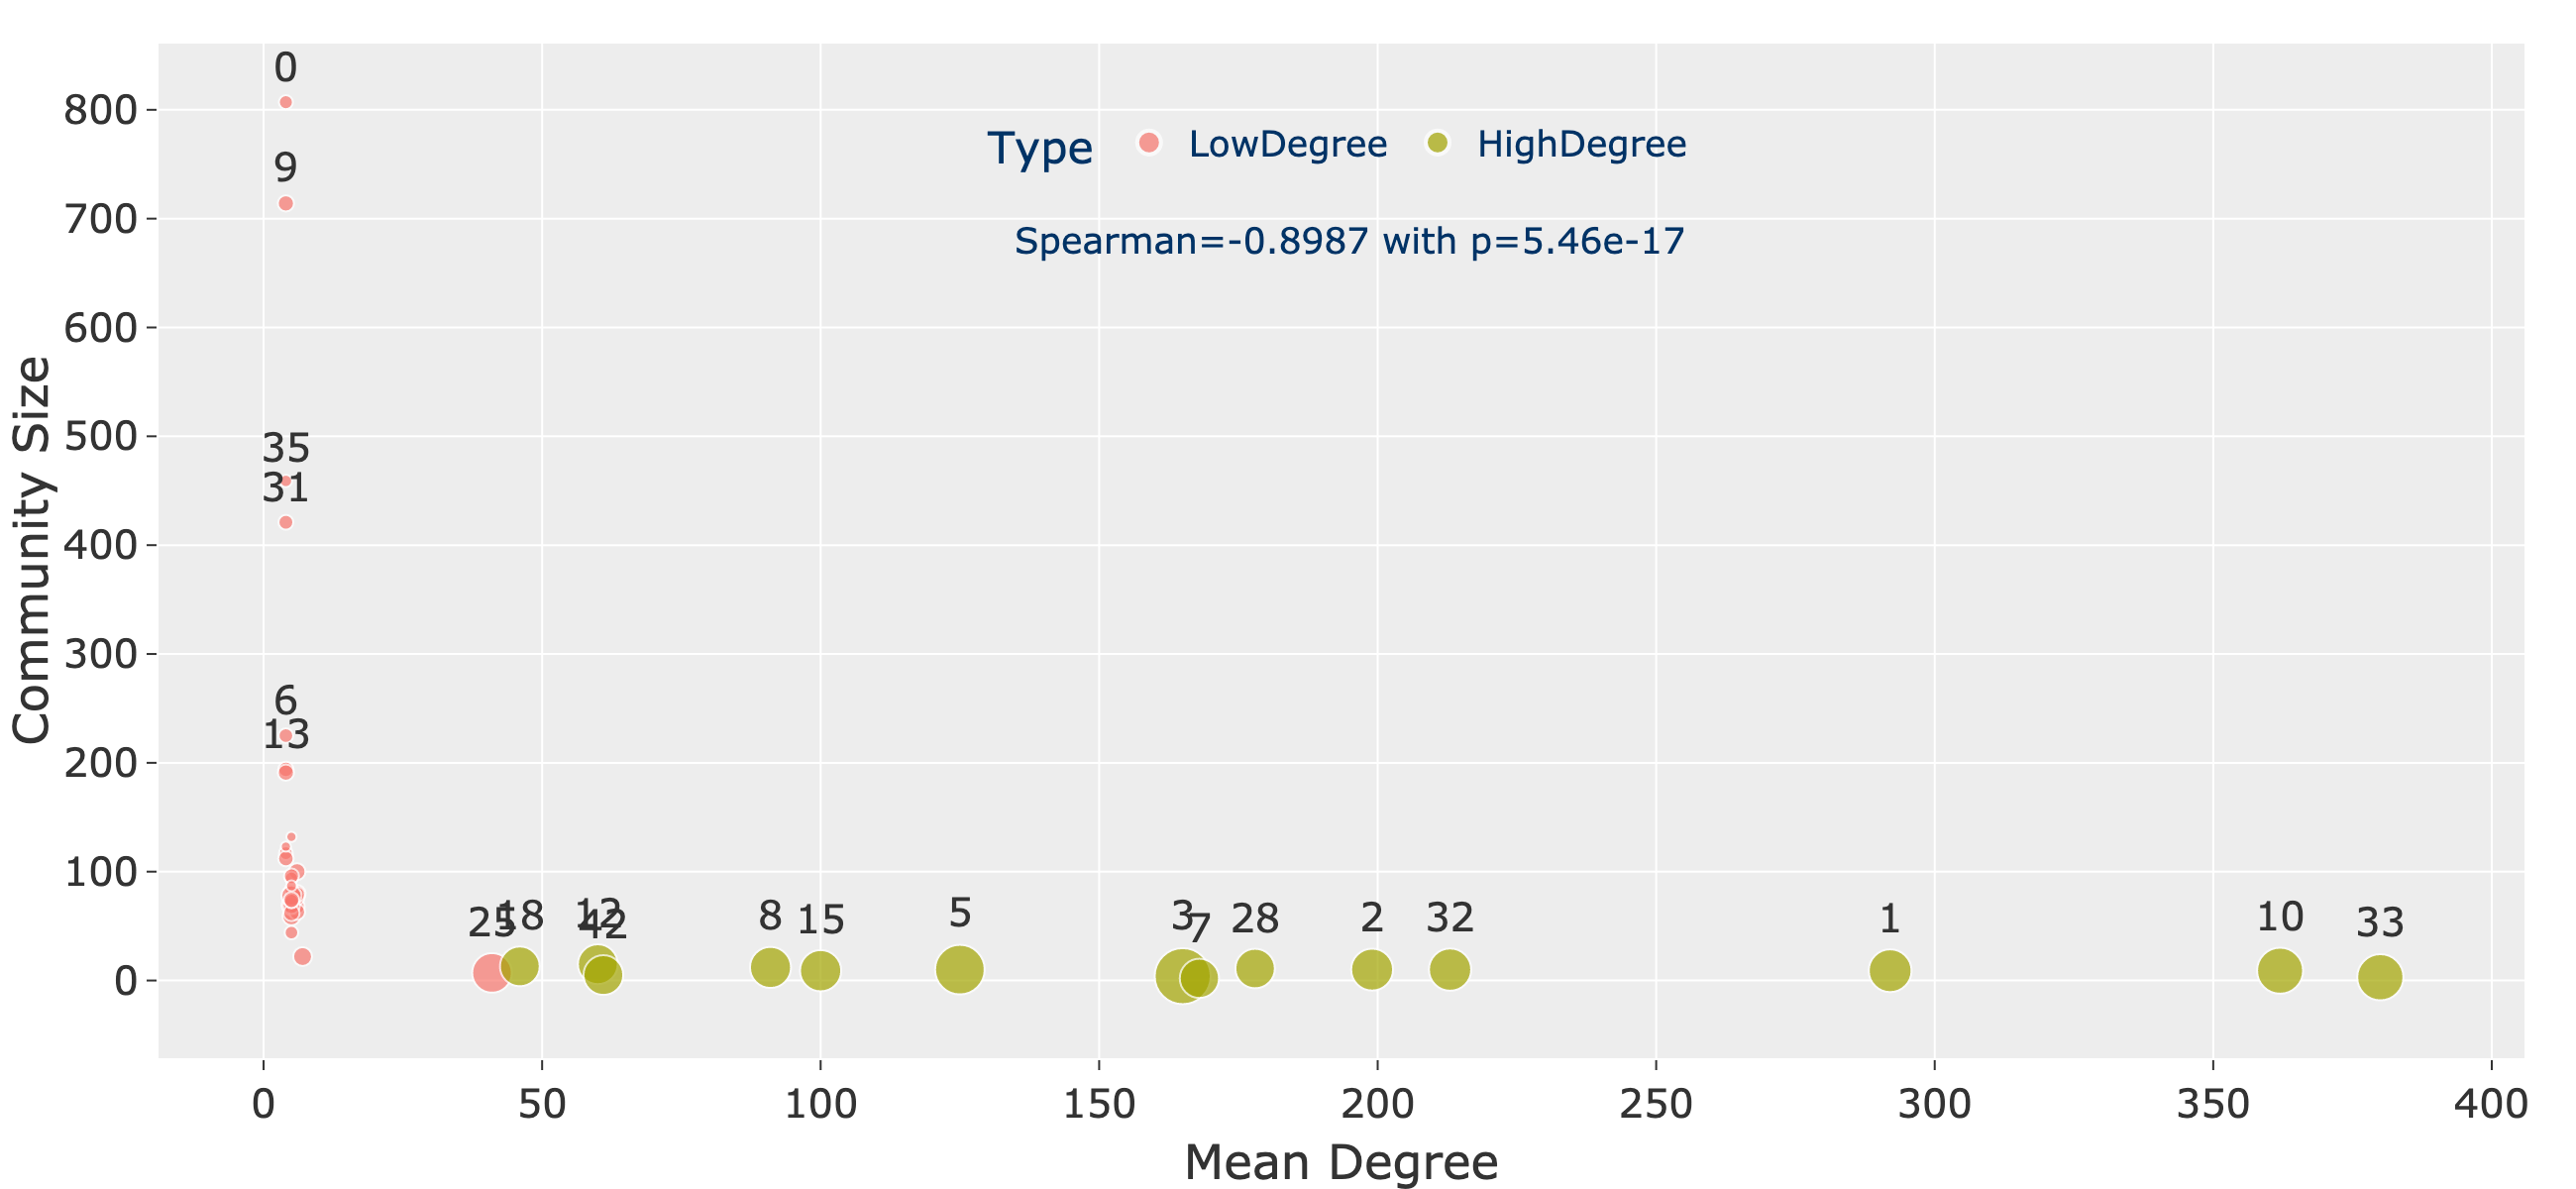
\includegraphics[width=1.0\textwidth,height=1.0\textheight,keepaspectratio]{Sections/Network_II/resources/reward/LargeSmall_com.png}
    \caption[Community size vs Degree]{Scatter plot showing the mean degree vs size of the communities found in the reward network. The marker size is proportional to the mean mutation burden in a community. The blocks are classified into two categories: 'HighDegree', which consists of the communities that have a mean degree in the top 30\%, and 'LowDegree', which includes the rest of the blocks. It can be seen that there is a direct correlation between community size and mean degree.}
    \label{fig:N_II:largeSmall_com}
\end{figure}

% Implication of the finding
This initial analysis demonstrates that the \acrlong{hsbm} effectively separates mutated genes with a high degree from the rest of the nodes. This suggests that the community detection method is capable of identifying very small communities, consisting of just a few nodes, from the 5000 genes used to construct the network. Furthermore, the unconnected genes are grouped together into larger clusters. The ability to find communities with fewer than 10 nodes indicates that \acrshort{hsbm} is capable of analysing larger networks, suggesting that the gene filtering threshold of 5000 could potentially be relaxed.

\subsubsection*{Understanding the group size imbalance}

% Discuss the source of this imbalance around the communities
These two observations attest the power of the community detection but do not explain the source cause of the size imbalance across communities. The analysis of the previous networks showed hints that there are a subset of nodes with a high but none of the weight modifier versions had such an effect as reward v2 to the networks. For example, genes in small, well-connected communities tend to have a high correlation even in an unmodified network; further explored in \cref{s:N_II:corr_rank}. 

% Example for AHR 
% Explaining what is happening
It is worth resurfacing that the selective edge pruning retains only the 3 or 6 top most correlated genes, which is why nodes like \textit{AHR} do not have a higher degree in the standard network. As the sigmoid modifier increases the correlation values of mutated genes, genes with reasonably high correlation but not among the top selected genes are affected.

The \textit{AHR} \acrlong{tf} which overexpression and mutation plays an important role in bladder cancer \citep{Shi2020-km}, is also correlated with the expression of other genes. As a TF the \textit{AHR} is allowed a minimum degree of 6 connections, and the rest of the edges need to come from the 'other genes'. In the standard network, \textit{AHR} is not among the top correlated values of these 'other genes', but with the sigmoid modifier, \textit{AHR} is pushed to the top. Thus, \textit{AHR} attains a higher degree. This example illustrates how the weight modifier and the community detection method group these highly connected nodes.

\begin{figure}[!t]    
    \centering
    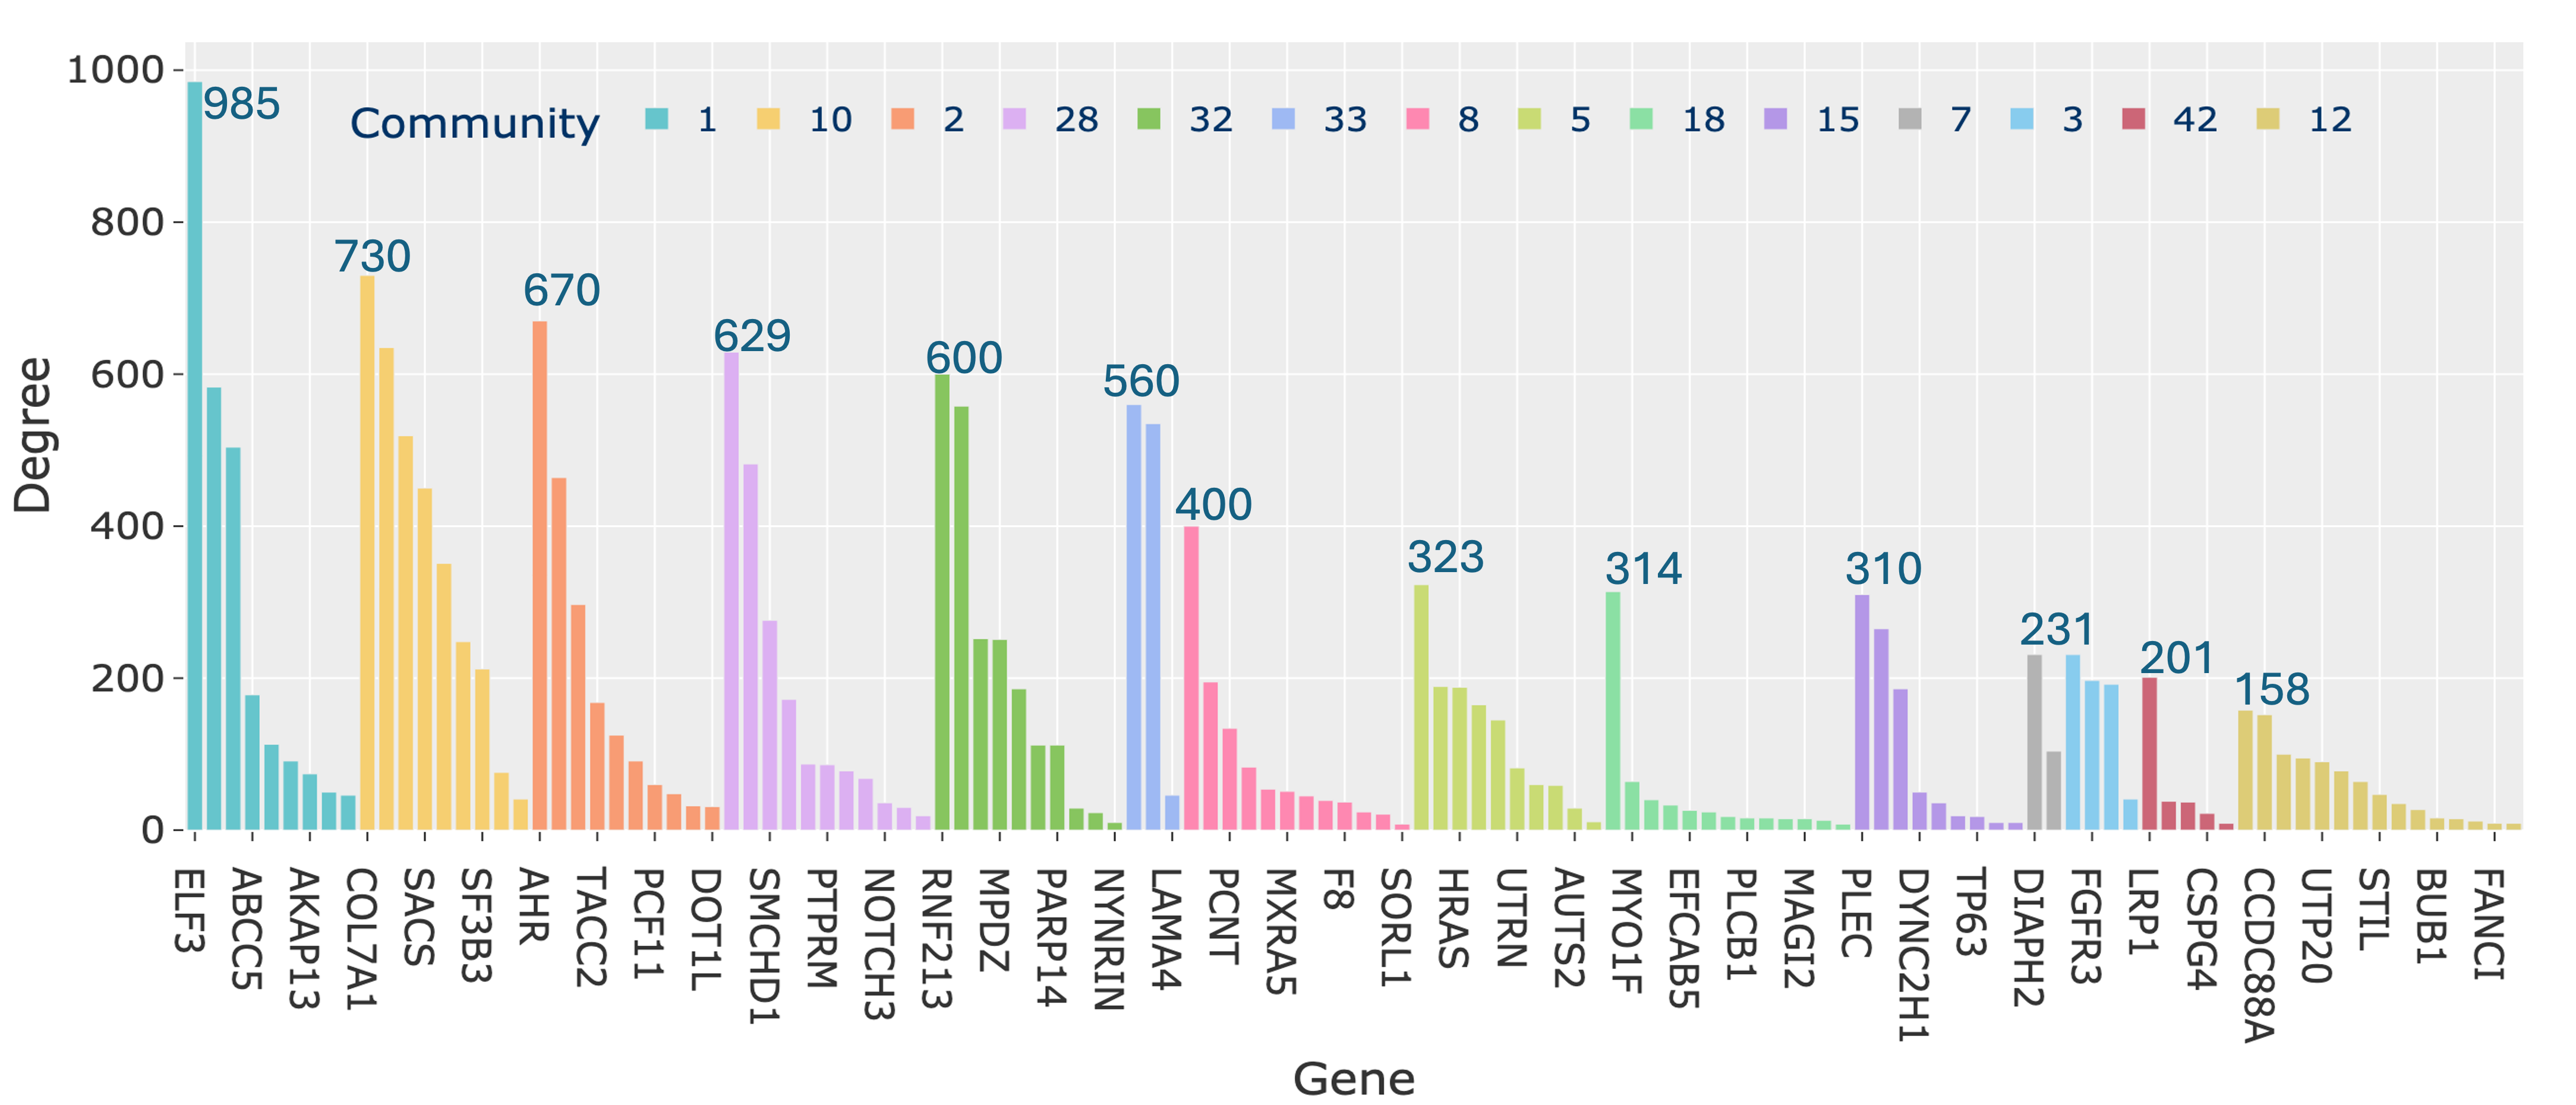
\includegraphics[width=1.0\textwidth,keepaspectratio]{Sections/Network_II/resources/reward/SmallCom_gene_labeled.png}
    \caption[Degree values of the highly connected genes]{The genes (X-axis) and their node degree (Y-axis) in the 14 highly connected communities; the colour is given by their community number. \textit{ELF3, AHR, FGFR3, TP63} are nodes with a high degree and genes which play a role in bladder cancer \citep{Robertson2017-mg} included in these groups showing that the network pipeline can isolate relevant genes based on the expression and their mutation burden.}
    \label{fig:N_II:genes_highConn}
\end{figure}


% Communities with high number of connections 
Out of the 45 communities found in the reward network, there are 14 which are in 70th percentile by group's mean degree. There are 122 genes across all these communities which are plotted on the X-axis in \cref{fig:N_II:genes_highConn} with the corresponding degree on the Y-axis, the bar plots are coloured by the community membership. The bar groups are ordered in descending order by genes' degree where the block with the highest mean degree on the left.


% Commenting on the plot
The most connected gene is \textit{ELF3} which is involved in bladder differentiation and is one of the Luminal Non-Specified markers from consensus \citep{Kamoun2020-tj} \& \cref{tab:lit:consensus_genes}. \textit{KLF5} which is the third highest connected gene in community 1 was shown in \cref{s:cs:basal_interp} to be differentially expressed to basal groups, and are associated with differentiation \citep{Bell2011-xj} and \cref{tab:N_I:markers_diff}. \textit{AHR} mutations are associated with bladder cancer \citep{Shi2020-km}, while \textit{FGFR3} is a known luminal marker \citep{Robertson2017-mg}. \textit{TP63} is also involved in bladder cancer \citep{Choi2012-kk, Karni-Schmidt2011-ps, Choi2014-ed} and controls cell cycle checkpoints.


% Highly correlated genes and the genes they contain
The 5000 nodes network is then filtered to display only the 14 communities in Appendix \cref{fig:ap:graph_smallCom}. The figure shows that there are communities consisting of only two or three genes. For example, community 7 contains two genes: \textit{ZFP36L2} and \textit{DIAPH2}. The former was found to promote cell aggressiveness in pancreatic cancer in a clinical study by \citet{Yonemori2017-ky} and was also identified through statistical analysis of TCGA's mutation data as a MIBC recurrence indicator by \citet{Han2019-ma}. The role of \textit{DIAPH2} is less known, but it has a high protein expression according to the \href{https://www.proteinatlas.org/ENSG00000147202-DIAPH2/tissue}{Human Protein Atlas}. Another group consists of \textit{LAMA4}, \textit{VPS13D}, and \textit{TRANK1}. The role of \textit{LAMA4} was studied in the context of gastric cancer, and up-regulating its expression led to treatment resistance according to \citet{Peng2020-xe}. The roles of the other two genes are less known. This suggests that the network pipeline is able to isolate both well-studied and potentially new genes into separate groups.


% Molecular properties
\subsection{High degree: mutations and correlations} \label{s:N_II:corr_mut_burden}

% Presenting the genes
So far a few known genes were mentioned in the analysis but it is unclear if the genes isolated in small communities were chosen by their correlation, mutation burden or both. The plot in \cref{fig:N_II:hist_molecular_highCon} attempt to answer this, by showing the mutation burden distribution of the highly connected genes versus the rest of the nodes in the network.

\begin{figure}[!b]    
    \centering
        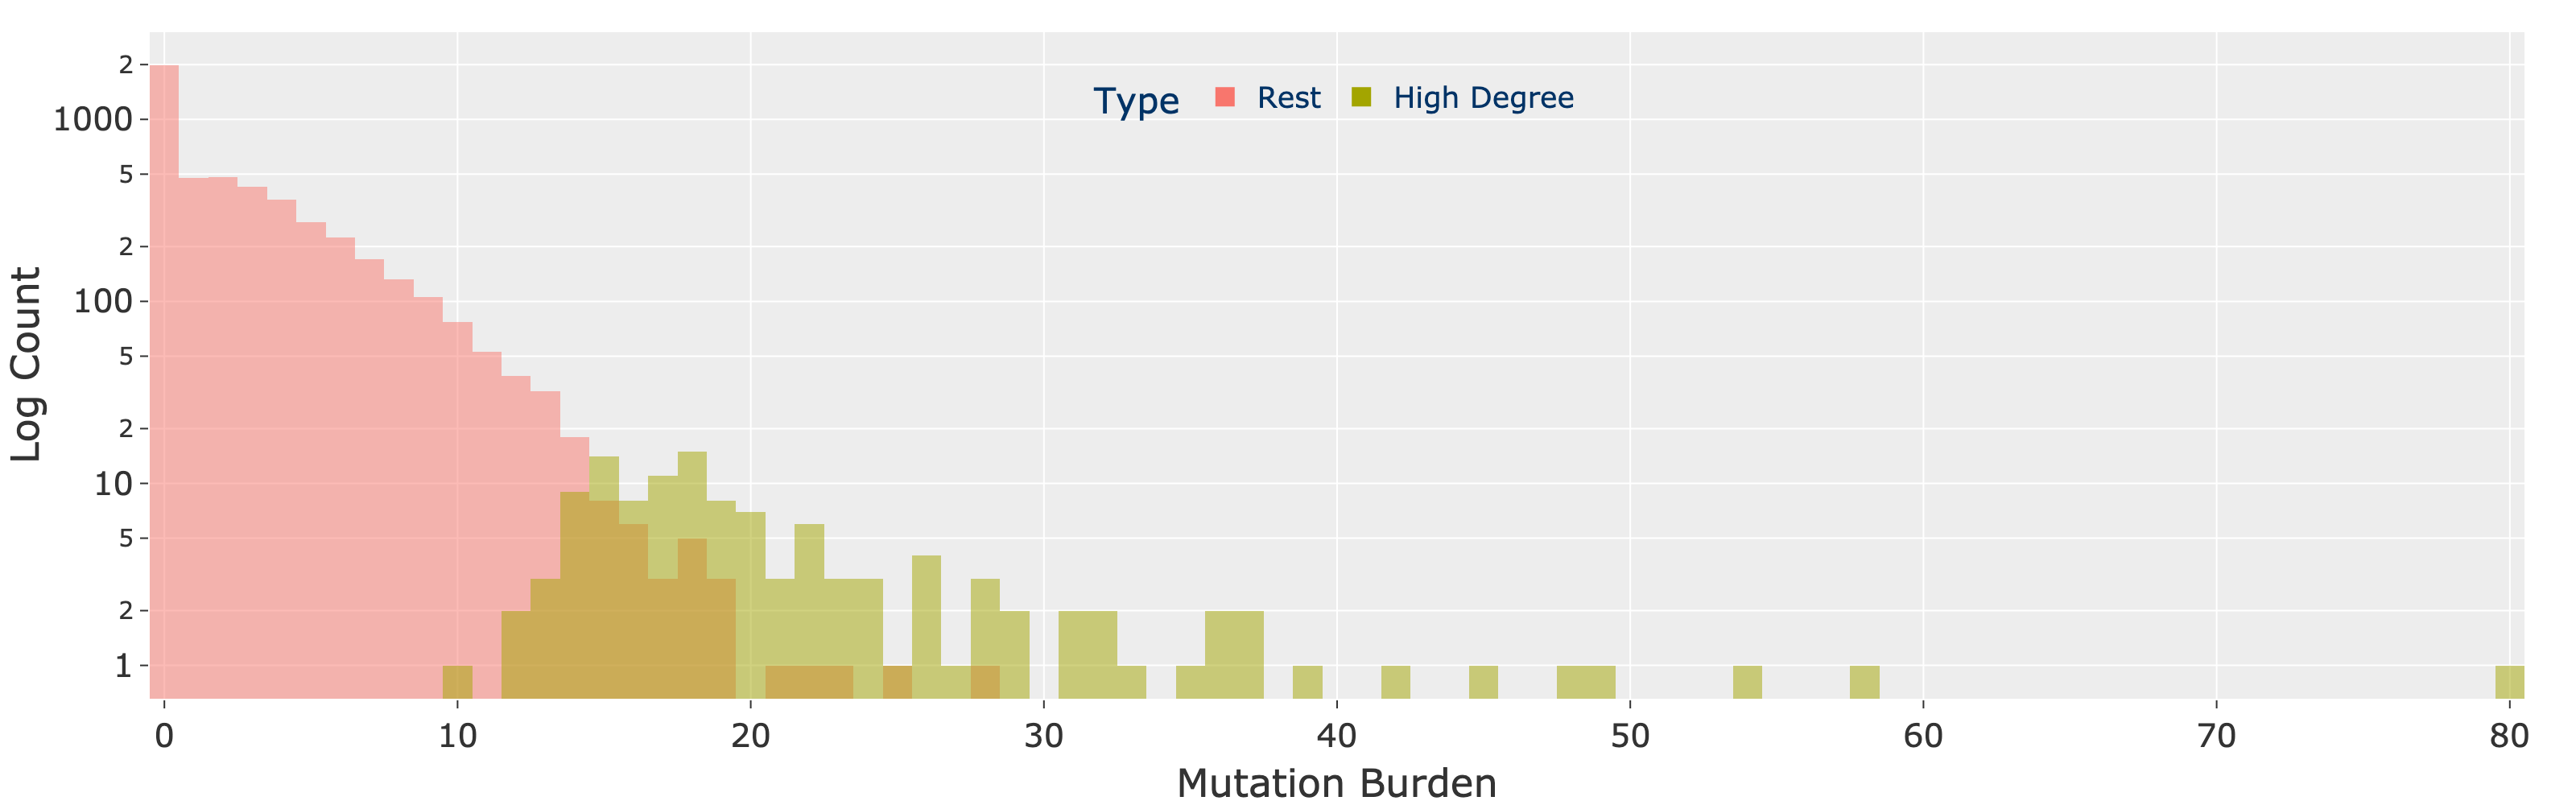
\includegraphics[width=1.0\textwidth,height=1.0\textheight,keepaspectratio]{Sections/Network_II/resources/reward/smallCom_MutHist.png}
        \caption[Mutation burden of the highly connected genes]{Distributions of the mutation burden across the high connected genes and the rest. The plot attests that that high degree communities exclusively contains mutated genes, further validating the data integration.}
        \label{fig:N_II:hist_molecular_highCon}
\end{figure}


% Commenting on the mutation burden 
The histogram from \cref{fig:N_II:hist_molecular_highCon} shows that all the genes in the 14 high degree communities are mutated in more than 10 samples across TCGA's MIBC cohort. It also shows that there are no highly mutated genes ($>$30) in the rest of the communities. This plot attests that that high degree communities exclusively contains mutated genes (\acrshort{mw}: 1928.5, p-value: $6.173e^{-84}$), further validating the data integration.

% Introduce that it is a difference
The two distributions in \cref{fig:N_II:hist_molecular_highCon} overlap between 10-30, where some of the genes with a mutation burden above 10 are not in the 70th percentile of the communities with the highest mean degree. This indicates that the the correlation values make the difference between the nodes with a higher degree and the rests. It is worth remembering that the nodes weights are the product between the weight modifier (i.e. mutation) and the Spearman correlation, which directly influences the number of connections in the selective edge pruning stage.

% Introduce the work to study the difference
To validate this hypothesis, the genes with mutations $\in[10,25]$ were selected to match the overlapping area in \cref{fig:N_II:hist_molecular_highCon}. For each of these nodes the Spearman values above 0.5 were kept which indicates that two genes are strongly correlated. The results are shown in \cref{fig:N_II:degree_high_corr}, where each circle is a gene with its size proportional to the mutation burden, the X values represents the number of correlations above 0.5 of the node with the other genes, and the Y values the number of degrees in the reward network; Y-axis is shown in log10. 

\begin{figure}[!b]    
    \centering
    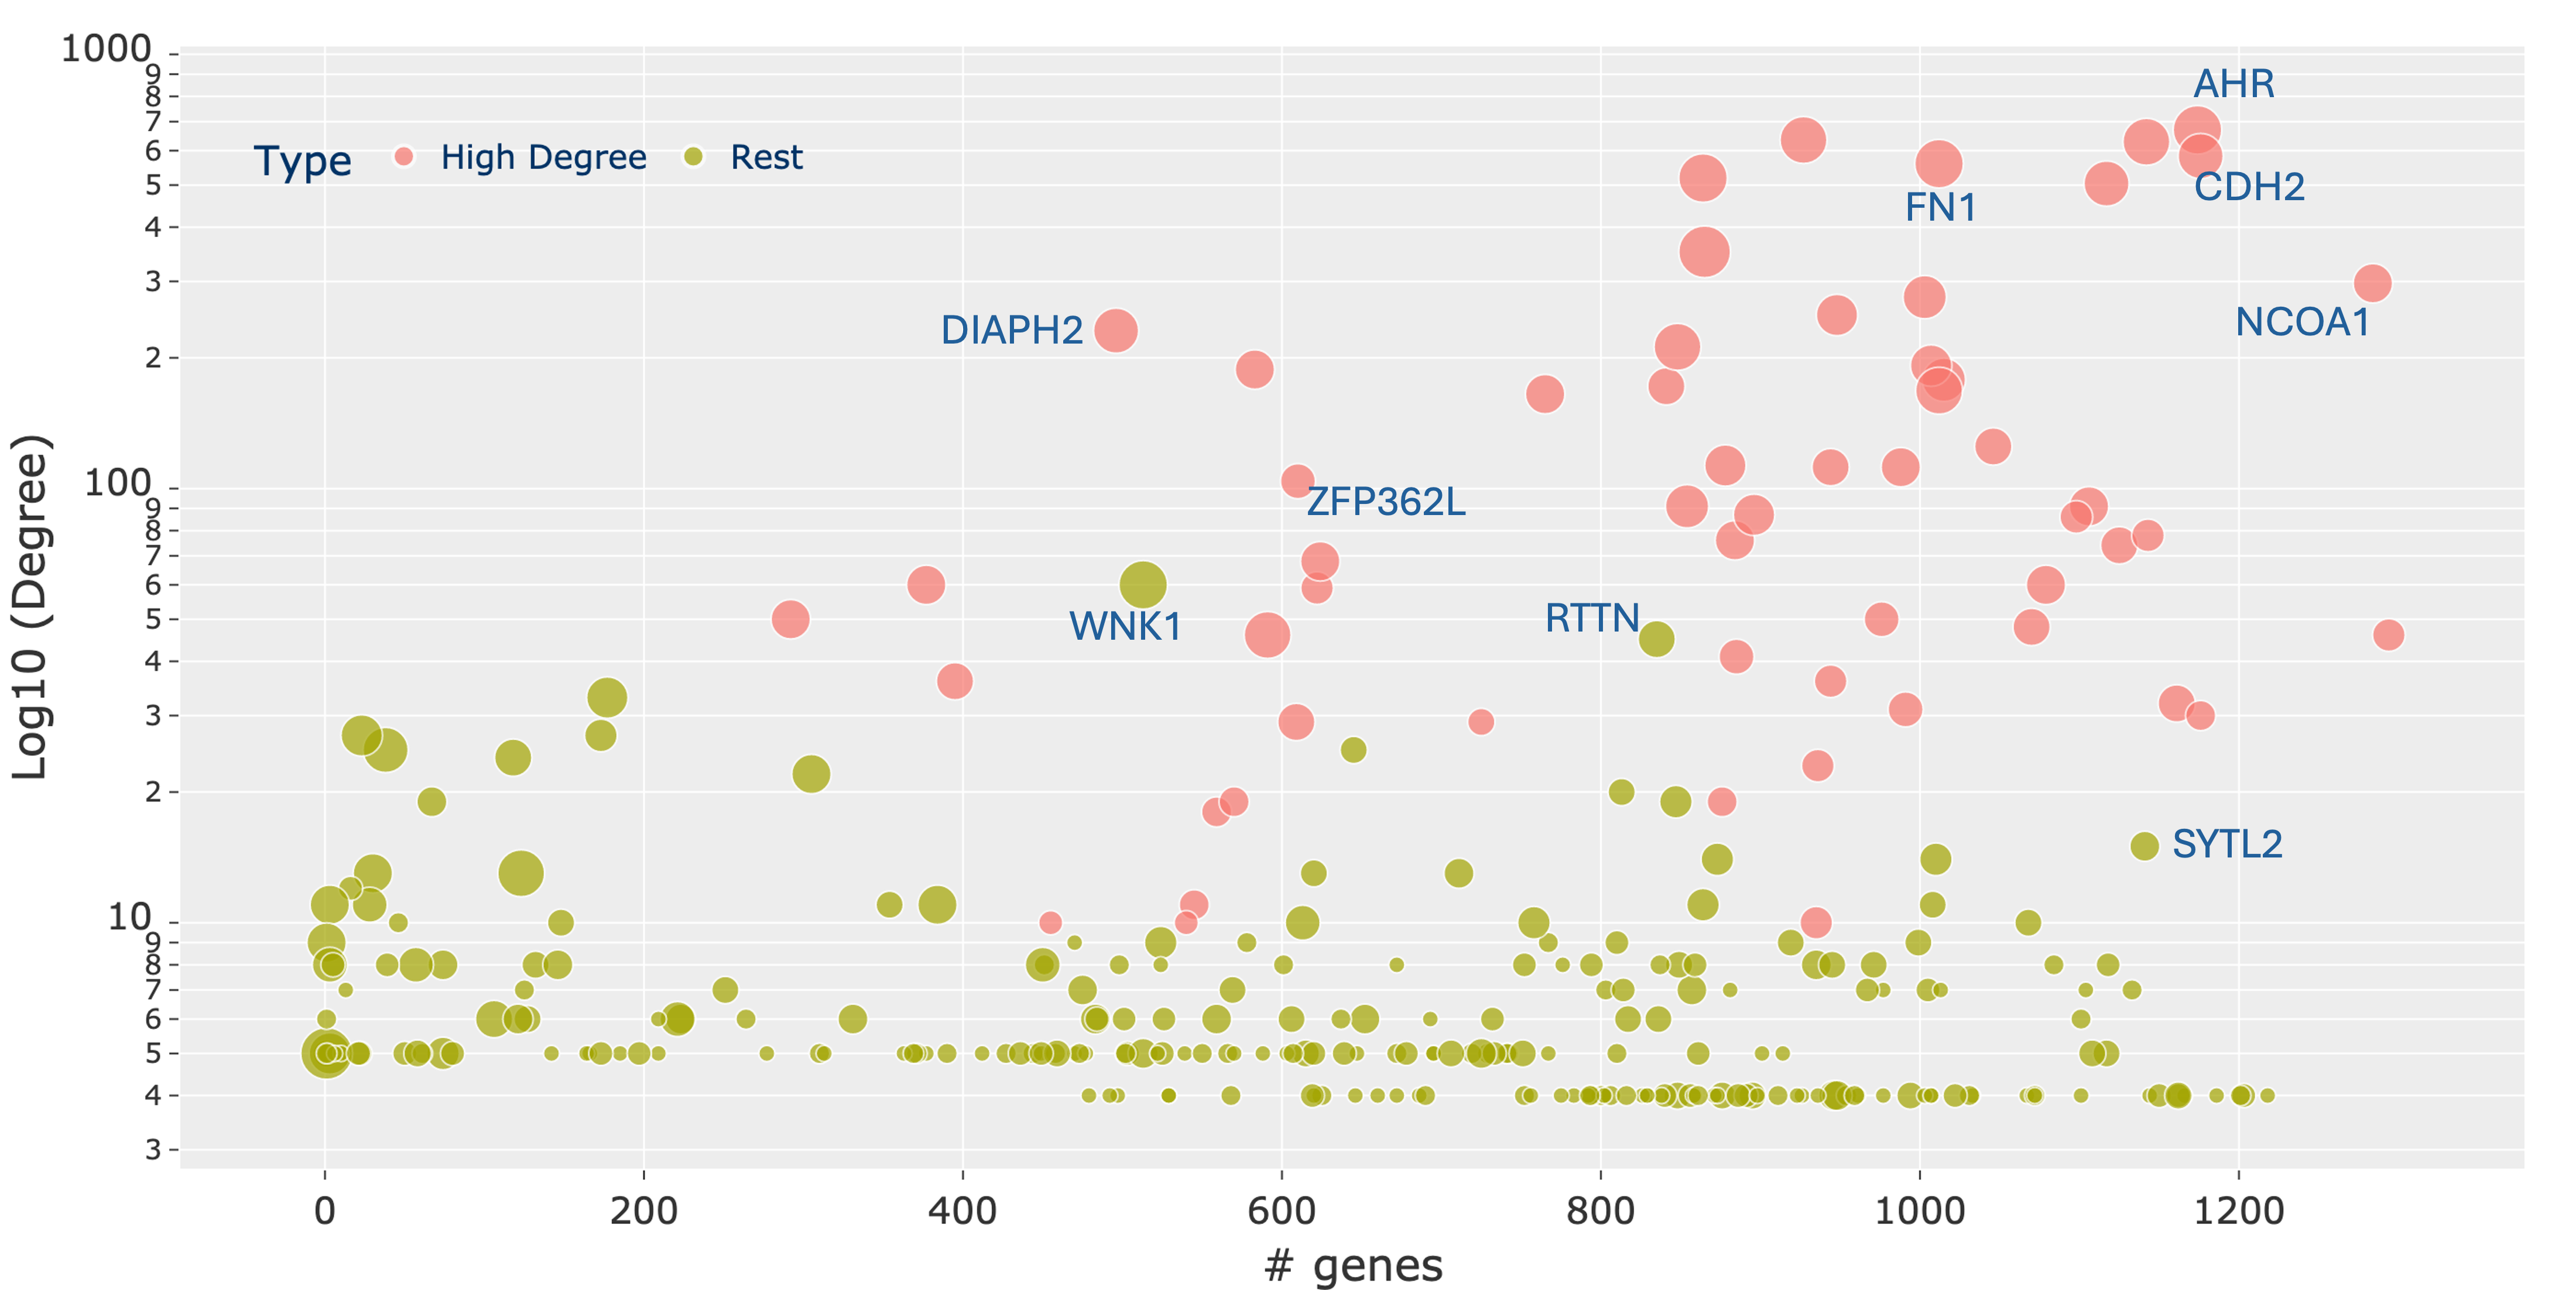
\includegraphics[width=1.0\textwidth,height=1.0\textheight,keepaspectratio]{Sections/Network_II/resources/reward/Degree_highCorrGenes_labeled.png}
    \caption[Number of connections vs their strength]{Scatter plot showing the genes with strong correlation (Spearman rank $>0.5$), where the Y-axis is the log10(degree), X-axis the number of correlations and the circle size is proportional to gene's mutation burden. The figure shows that the high degree nodes also have a large number of strong correlation and a high mutation burden. }
    \label{fig:N_II:degree_high_corr}
\end{figure}


% Comment the plot 
The top-right corner in \cref{fig:N_II:degree_high_corr} contains the nodes that are the most connected and have the highest number of correlations above the threshold, while the diagonally opposite corner contains low-correlated genes with few connections. The scatter plot shows that all the markers in the top-right corner are genes with a high number of connections, while in the opposite corner, such nodes are absent. In the bottom-left corner, there are a few genes with a high mutation burden (large circle), but due to the small number of highly correlated genes, the reward modifier does not have enough power to include them in communities with a high mean degree. Conversely, in the bottom-right corner, where there are several markers close to the X-axis, these genes do not have a high mutation burden to obtain more connections. This confirms that the number of connections is a function of both the correlation values and the mutation burden. There distributions of the degree values of the "High Degree" and "Rest" are significantly different (\acrshort{mw}: 565.5, p-value: $6.546e^{-43}$), as well as the mutation burden (\acrshort{mw}: 8484.0, p-value: 0.0001).

% The exception
While \cref{fig:N_II:degree_high_corr} confirms that the number of connections is a function of both the correlation values and the mutation burden of the genes, there are a few exceptions such as \textit{WNK1}, \textit{RTTN}, and \textit{SYTL2}. These genes exhibit a high number of correlations above 0.5 and a relatively higher number of connections but are not part of the 14 communities with a high mean degree. These exhibit significantly different correlation distributions (\acrshort{kw}: 555.026, p-value:$5.654e^{-120}$), along with \textit{AHR}'s, are displayed in \cref{fig:N_II:corr_sel_genes}. 


\begin{figure}[!b]    
    \centering
    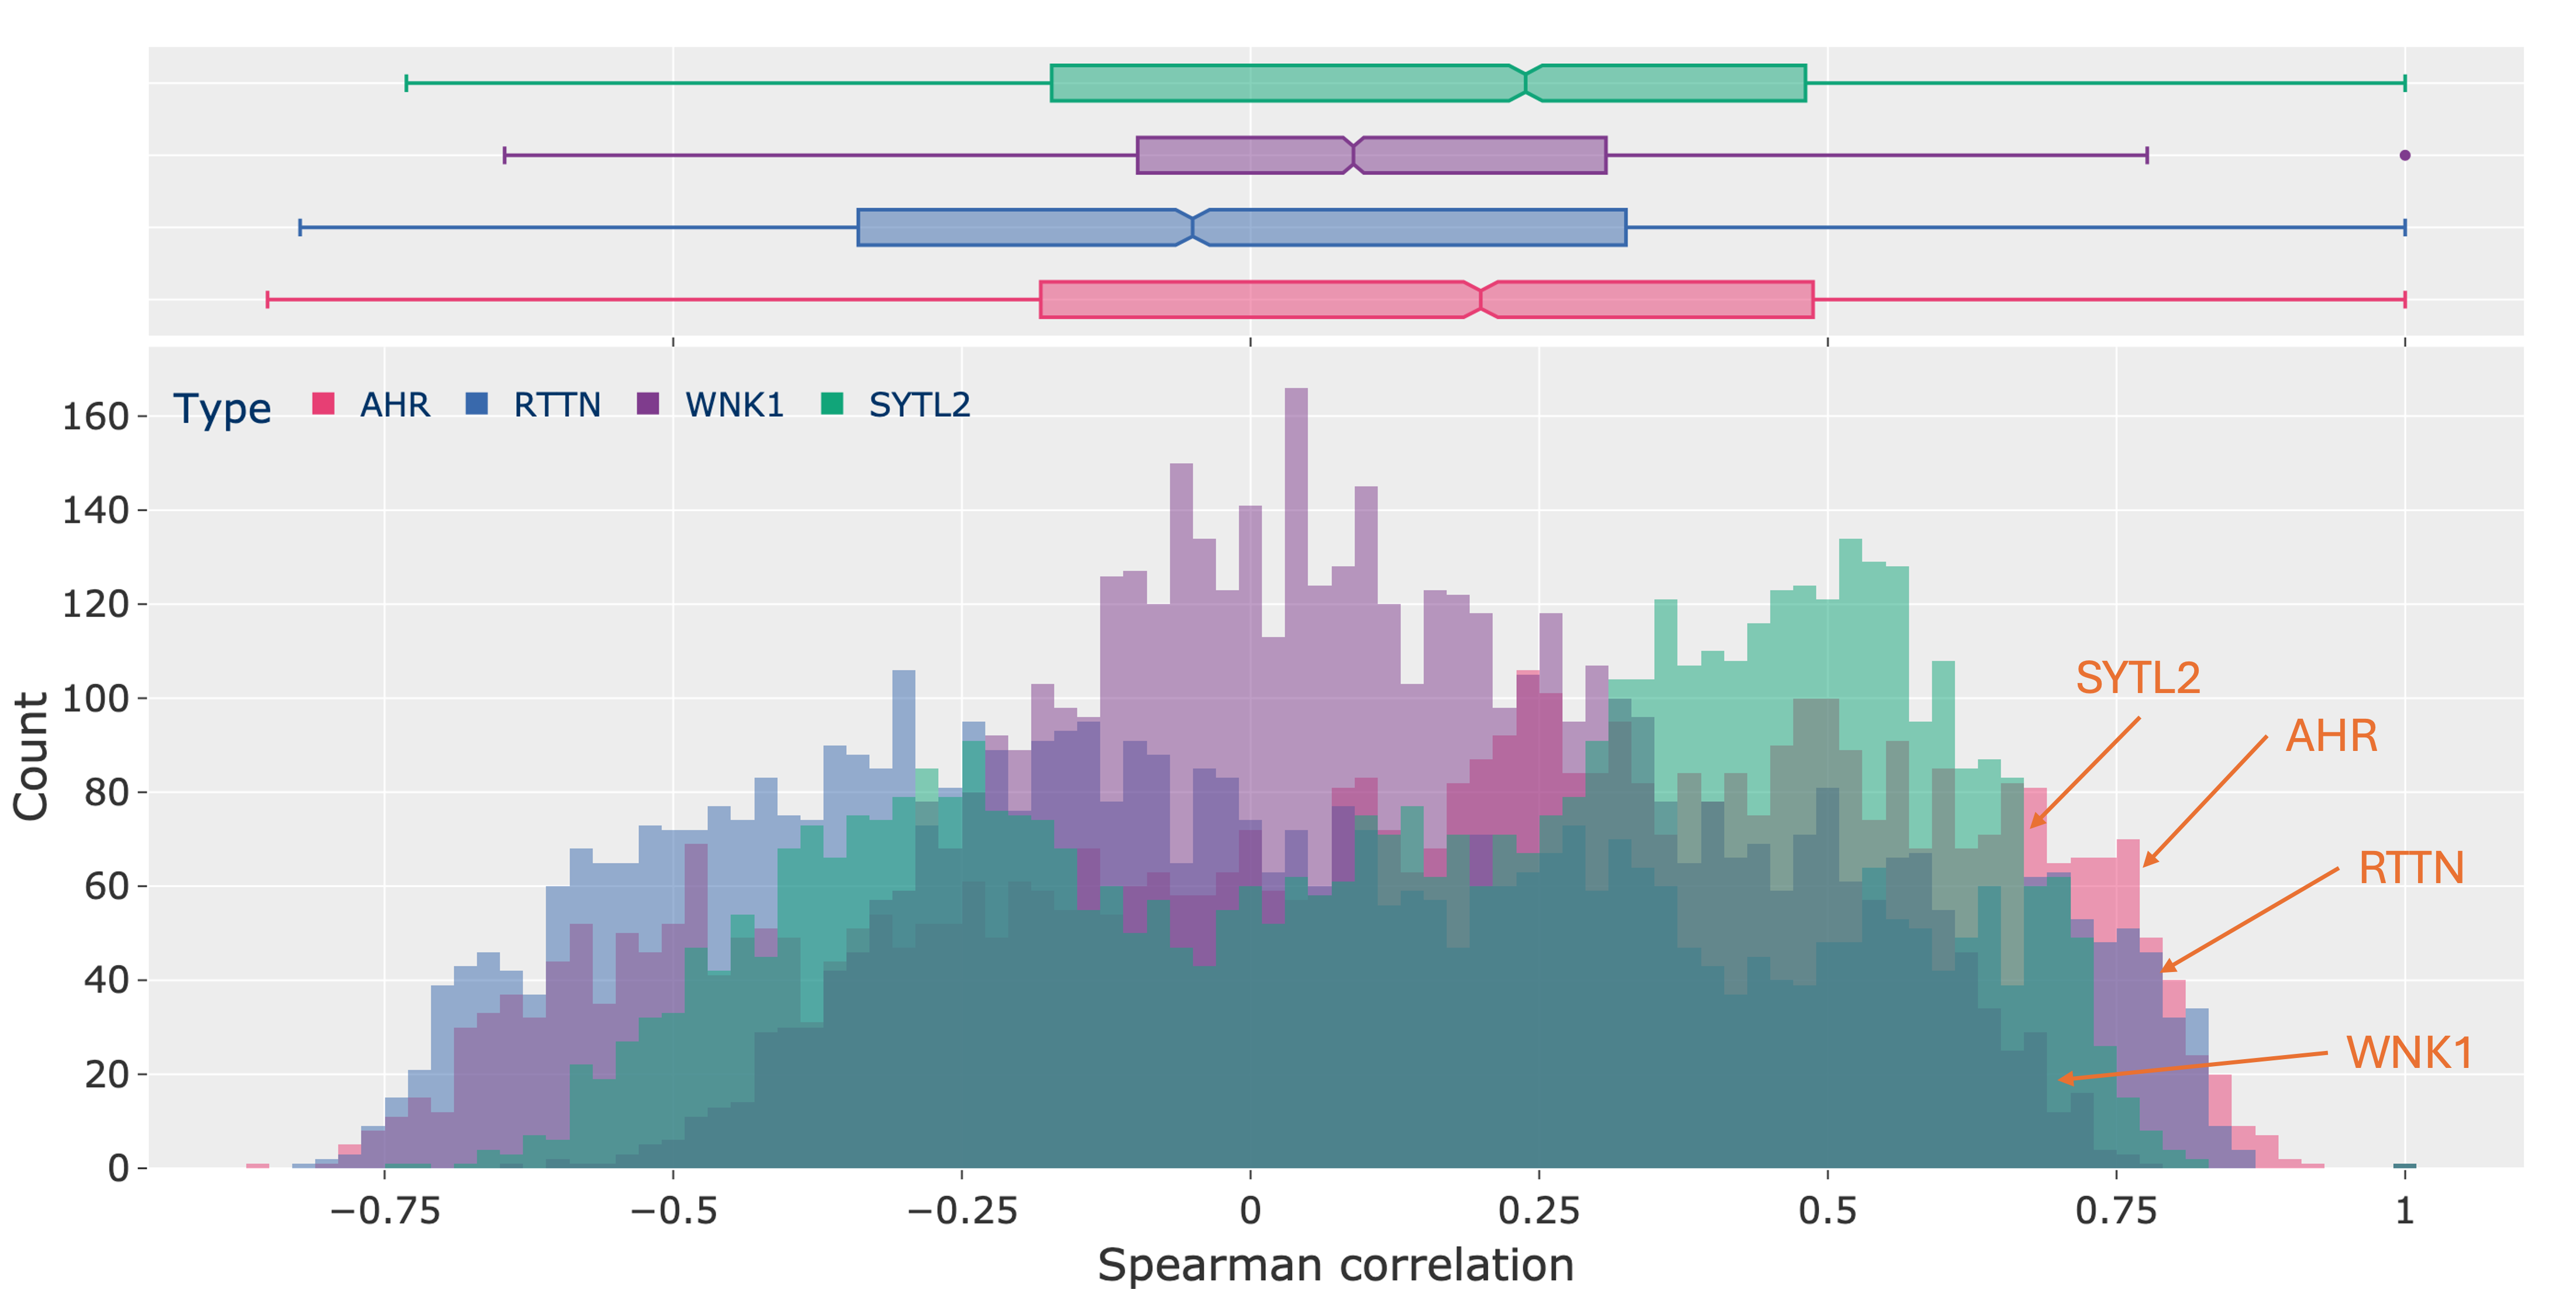
\includegraphics[width=1.0\textwidth,height=1.0\textheight,keepaspectratio]{Sections/Network_II/resources/reward/hist_corr_labels.png}
    \caption[Distribution of Spearman for a few genes]{Histogram of the Spearman correlation distribution of \textit{WNK1, SYTL2, RTTN}, and \textit{AHR}. The focus in this figure is on the values above 0.5, denoting the number of nodes to which the 5 genes have a good correlation. Both \textit{SYTL2} and \textit{AHR} have a large number of genes with correlation $>$0.5 compared to the other two, and the former has more values above 0.75. }
    \label{fig:N_II:corr_sel_genes}
\end{figure}


% Talk about the histrogram
The histogram indicates that \textit{AHR} and \textit{SYTL2} show more correlations with values above 0.5, as evidenced by the box plot at the top and the X-values in \cref{fig:N_II:degree_high_corr}. Although these two genes have similar distributions, it is noticeable that \textit{AHR} has a higher mutation burden (23 - \textit{AHR} and 14 - \textit{STYL2}) a greater number of correlations exceeding 0.75, leading to stronger weights. In contrast, \textit{WNK1} and \textit{RTTN} have correlation values that are centred around 0 (\textit{WNK1}) or are skewed to the left (\textit{RTTN}), indicating a tendency towards weaker or negative correlations.

The two plots, \cref{fig:N_II:degree_high_corr,fig:N_II:corr_sel_genes}, confirm that the data integration has an impact on the network and that genes with a high number of connections need to have both a high number of correlations and a high mutation burden. It also shows that the labelling of some genes depends on the weight magnitude, as some genes are not included in the 14 communities with a high mean degree.




% Correlation rank
\subsection{High degree: correlation rank} \label{s:N_II:corr_rank}

% Introduce what I am going to talk about
It is clear that the reward modifier successfully integrates the mutation burden into the co-expressed gene network. However, it is not clear how the sigmoid function affects the correlation raking, how the values above a certain threshold are influenced to give a node a few hundreds connections when each gene is allowed to keep either the 3 or 6 most correlated genes.

% Why it is important to understand this change
In the case of the 122 highly degree nodes, the rest of the connections must come from their neighbours to contain the subset of 122 genes in their top correlation. For example, the most connected gene \textit{ELF3} (a TF) has 985 neighbours and only 6 are being in the gene top correlation. The rest of the 979 gene have \textit{ELF3} in their top ranking. It is important to verify if the 979 genes have \textit{ELF3} already high in their correlation ranking before the reward modifier is applied as it will mean these genes have a weaker co-expression that is only amplified with the reward.

\begin{figure}[!t]
    \centering
    \begin{subfigure}{0.49\linewidth}
        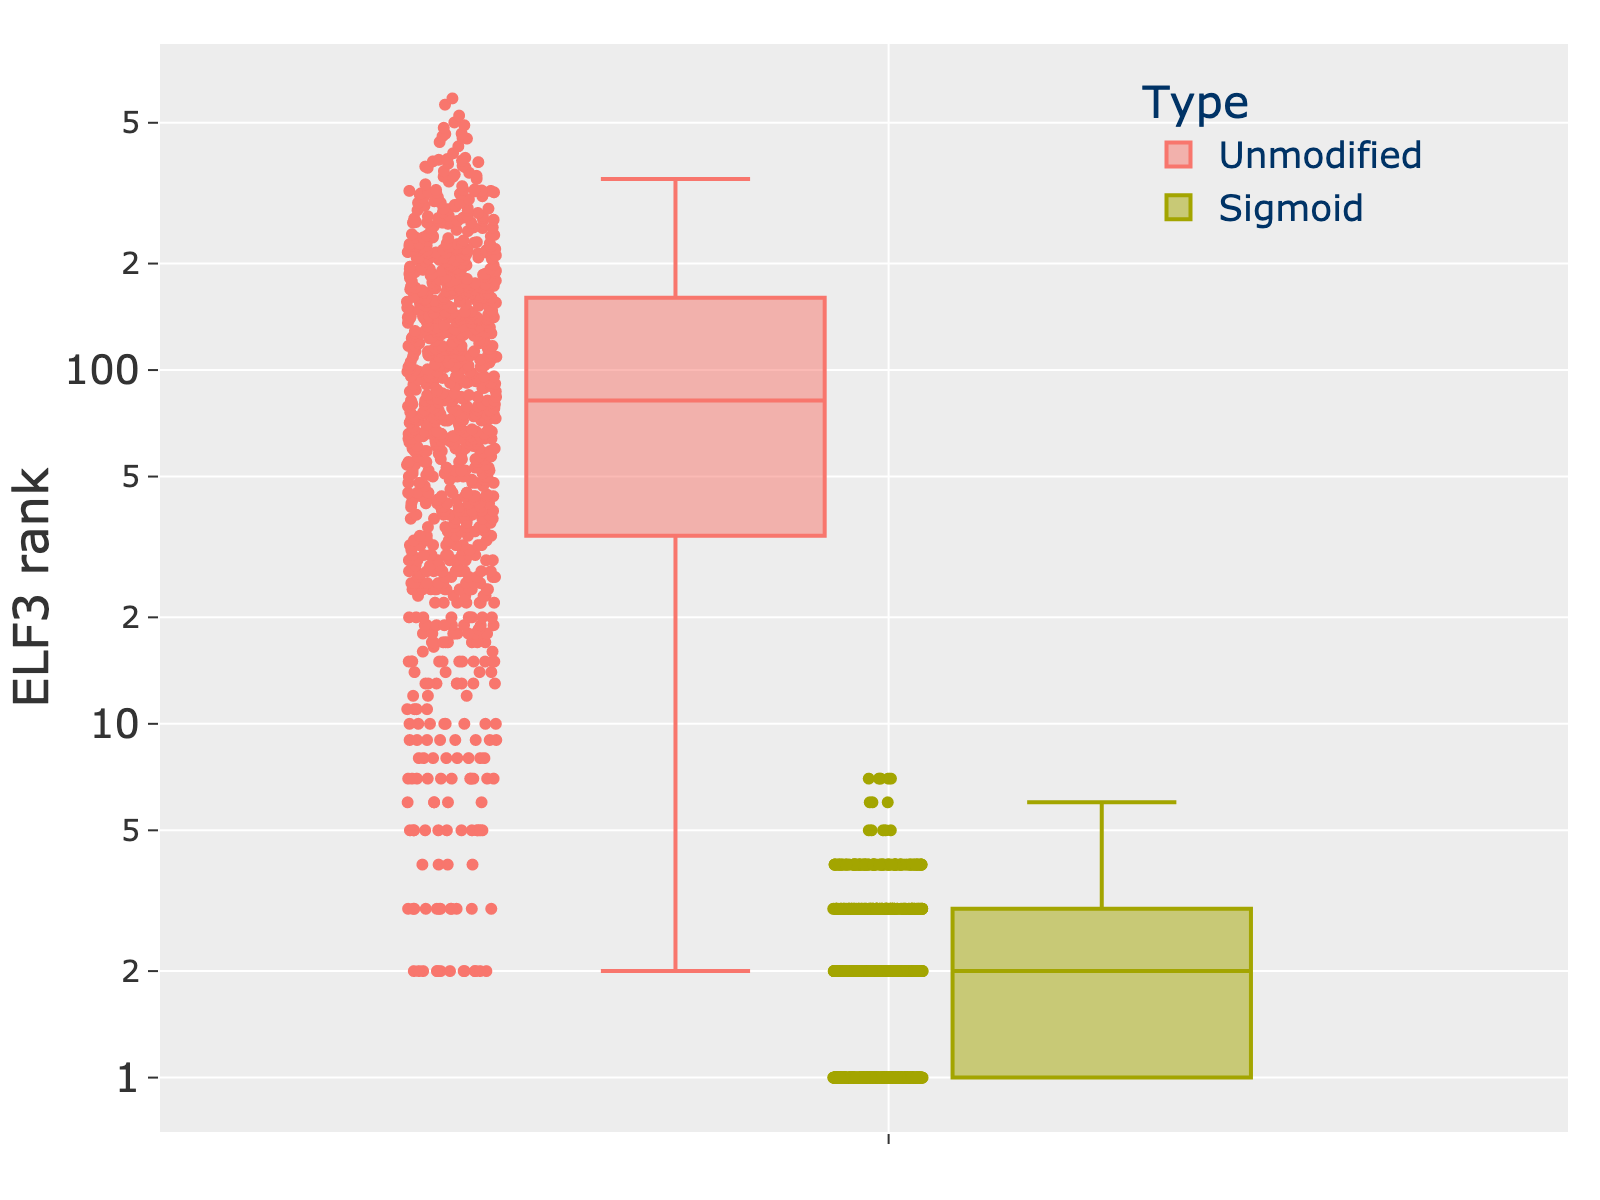
\includegraphics[width=1.0\textwidth,height=1.0\textheight,keepaspectratio]{Sections/Network_II/resources/reward/corr_analysis/ELF3_box.png}
        \caption{ELF3}
        \label{fig:N_II:ahr_corr}
    \end{subfigure}
    \centering
    \begin{subfigure}{0.49\linewidth}
        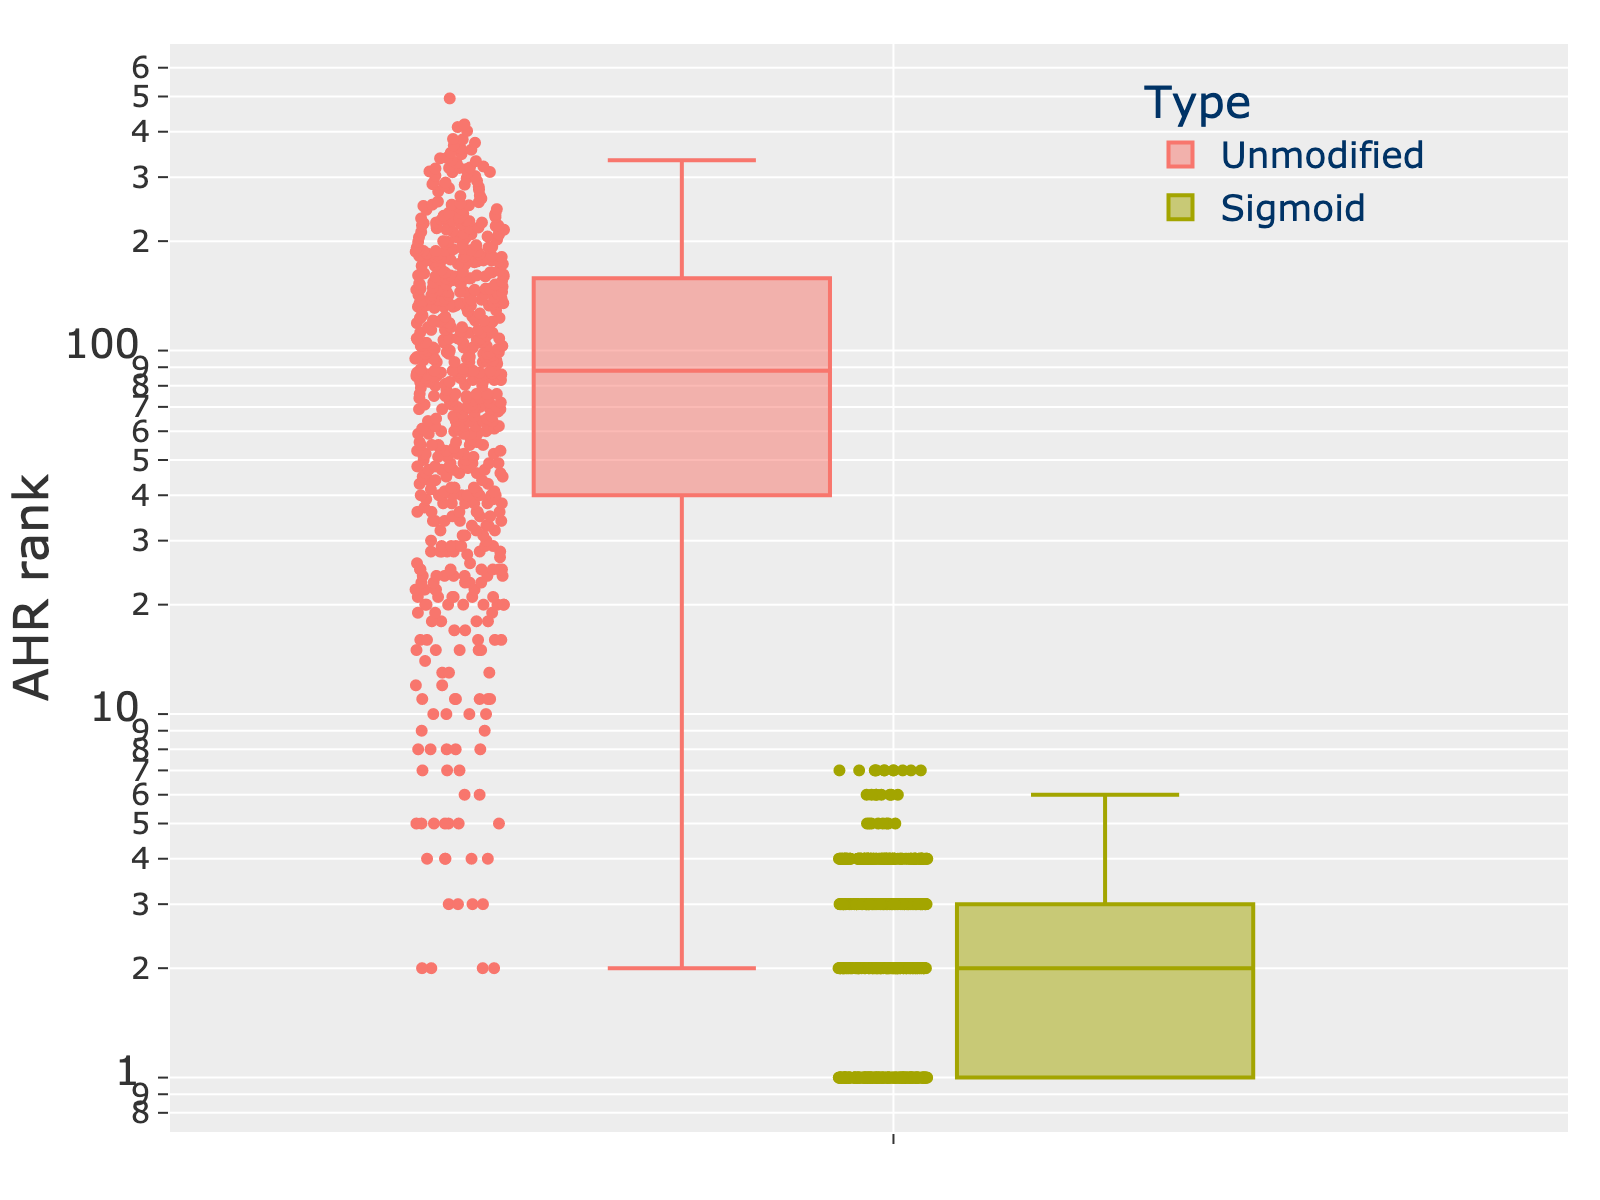
\includegraphics[width=1.0\textwidth,height=1.0\textheight,keepaspectratio]{Sections/Network_II/resources/reward/corr_analysis/AHR_box.png}
        \caption{AHR}
        \label{fig:N_II:elf3_corr}
    \end{subfigure} %
    \centering
    \begin{subfigure}{0.49\linewidth}
        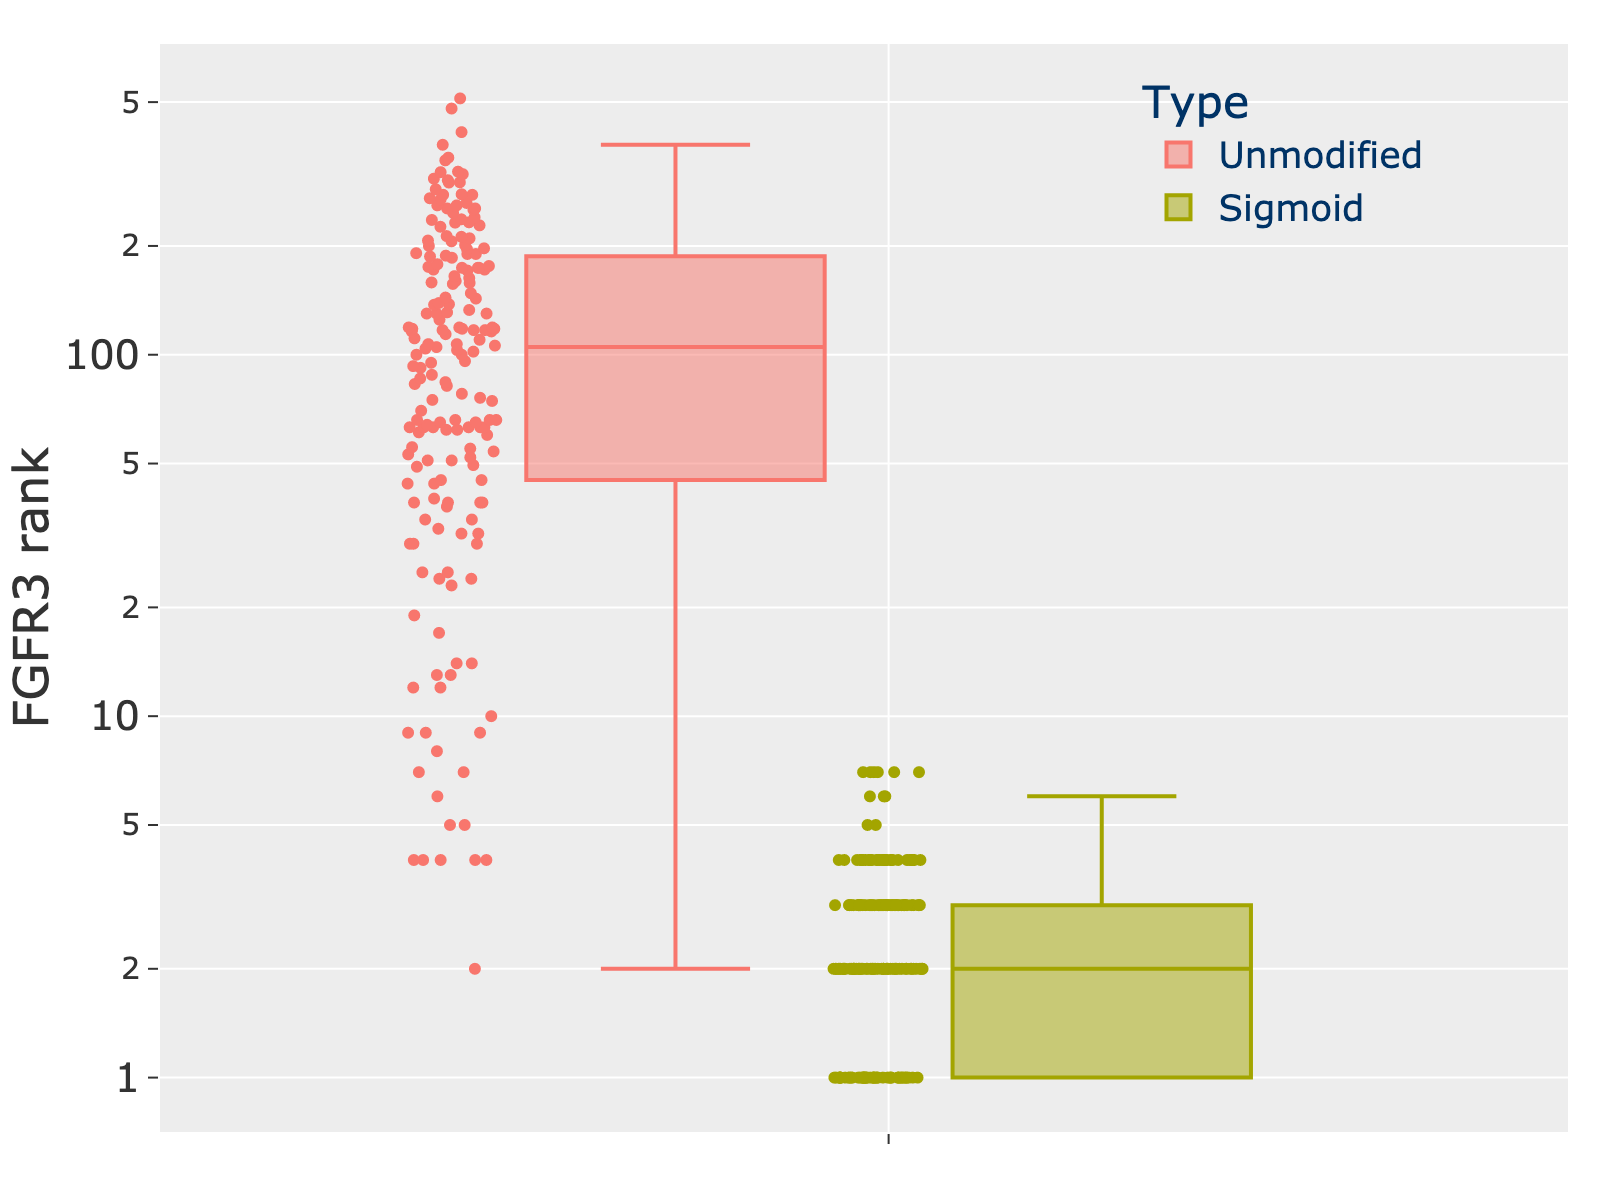
\includegraphics[width=1.0\textwidth,height=1.0\textheight,keepaspectratio]{Sections/Network_II/resources/reward/corr_analysis/FGFR3_box.png}
        \caption{FGFR3}
        \label{fig:N_II:fgfr3_corr}
    \end{subfigure}
    \begin{subfigure}{0.49\linewidth}
        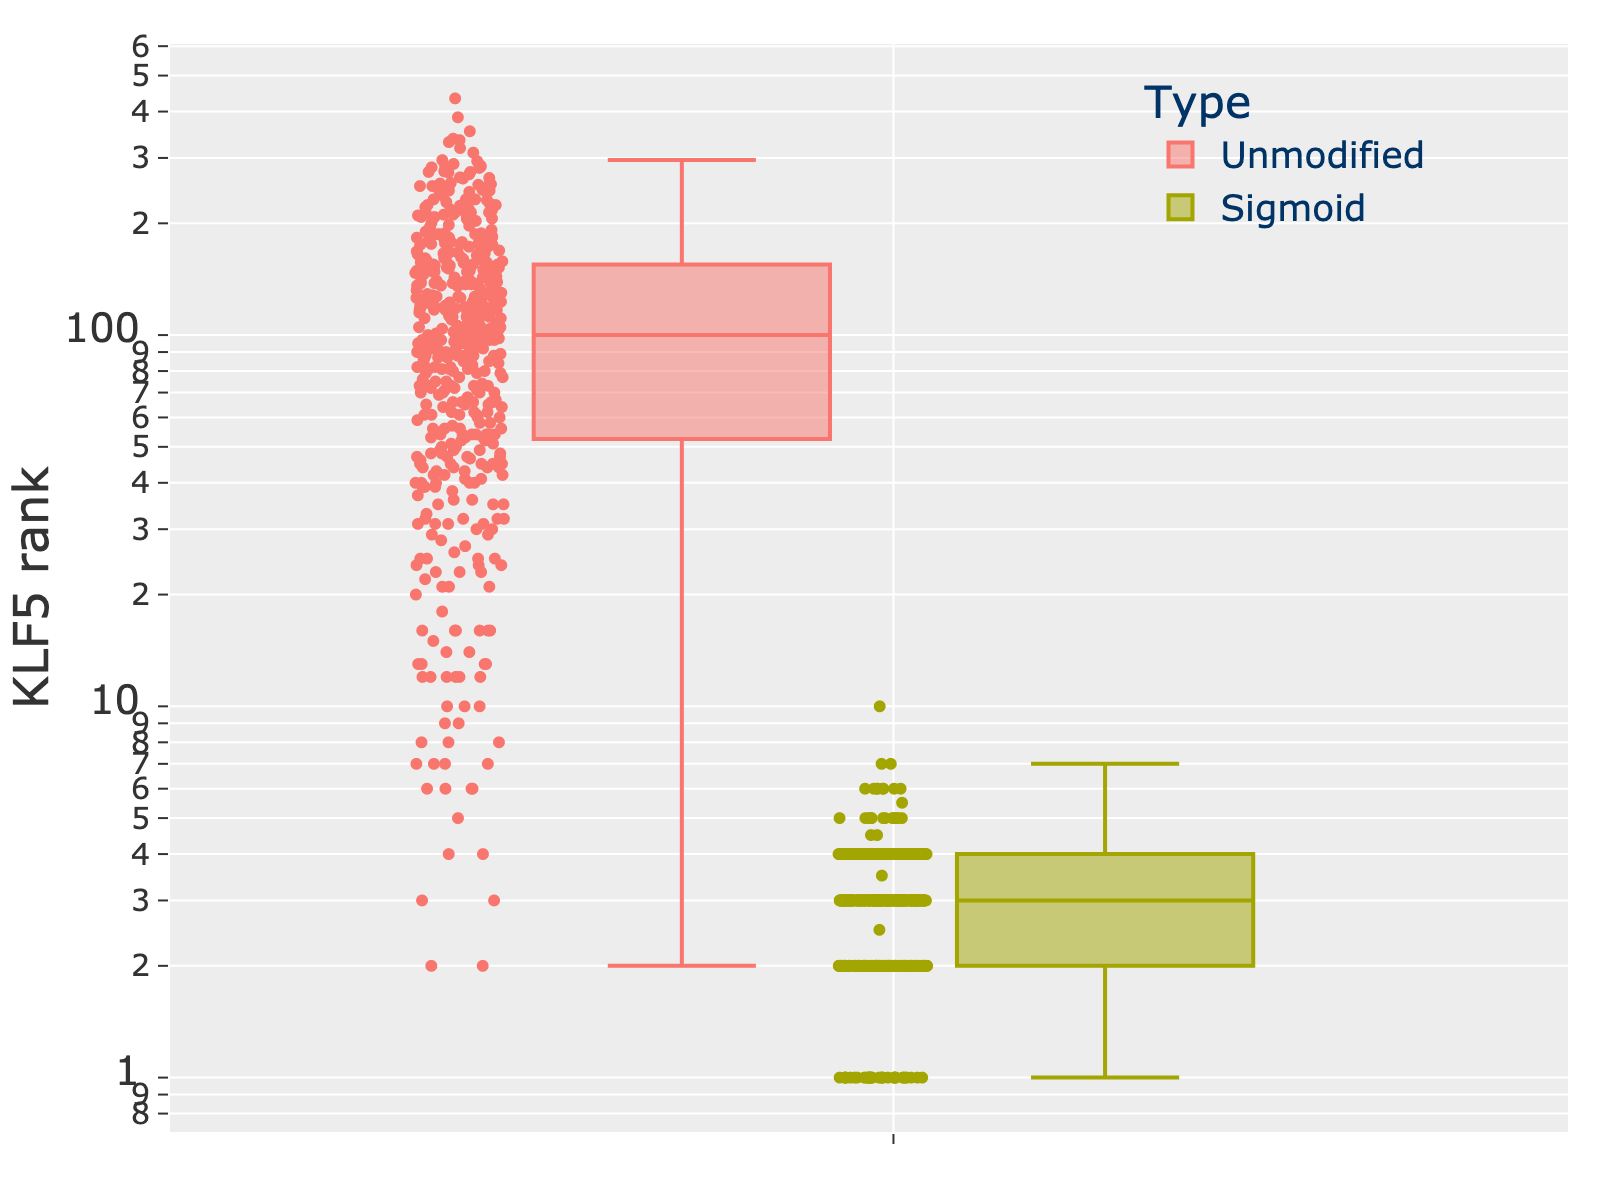
\includegraphics[width=1.0\textwidth,height=1.0\textheight,keepaspectratio]{Sections/Network_II/resources/reward/corr_analysis/KLF5_box.png}
        \caption{KLF5}
        \label{fig:N_II:klf5_corr}
    \end{subfigure}
    \caption[Spearman ranks of neighbour genes]{Each point in the box plot represents the rank in the Spearman correlation matrix for neighbours of four high-degree genes: \textit{ELF3}, \textit{AHR}, \textit{FGFR3}, and \textit{KLF5}. The red points indicate the unmodified correlation matrix, while the mustard points represent the ranks in the reward-modified correlation matrix (using the sigmoid function). A gene is considered a neighbour if it has a direct connection with the gene being studied (e.g., \textit{AHR}). The higher a neighbour gene ranks, the more strongly it is co-expressed with the studied gene. The four box plots show that in the unmodified network, the neighbour genes of high-degree nodes tend to have lower ranks. However, after applying the sigmoid reward modifier, these neighbours are boosted to higher ranks, leading to an increased number of connections for a select few nodes.}
    \label{fig:N_II:corr_analysis}
\end{figure}


% Explain the correlation rank plots
To understand this effect to a gene (e.g. \textit{ELF3}), the nodes that are directly connected to \textit{ELF3} in the reward network are 'extracted' as neighbour genes. For each of this gene it is computed the ranks in both the unmodified Spearman correlation matrix and the one modified by the reward modifier. Then the rank of the \textit{ELF3} gene is extracted, thus giving a relative indication of how well the two genes are connected.

% Introduce the plots
The ranks from both the Spearman correlation (red) and matrix changed  by the reward modifier (green) are shown for \textit{ELF3, AHR, FGFR3} and \textit{KLF5} gene in \cref{fig:N_II:corr_analysis}. All of these four genes have a well known function in the bladder tissue, are mutated and are high degree nodes. The four figures show that all the ranks in Spearman correlation matrix have a high variance and the four genes are usually within the top $\sim15$\% (rank $500-600$) of the neighbour's ranking. In addition, the ranks for the reward modified matrix are in 1-7 range\footnote{With the exception of the gene \textit{NCOA1}, in the box plot for \textit{KLF5}, which has in its ranks the \textit{KLF5}. Thus, both genes have each other in their higher correlation ranks.} showing the clear effect on the correlation ranks after the reward modifier is applied. 

% Control
\subsubsection*{Control} \label{s:N_II:ctrl_exp}

To appreciate the chances of the 122 genes being selected by just the mutation burden, a control network was generated. In this graph, the 122 genes were all assigned a mutation burden of 0, while 122 not-mutated genes (i.e., control gene) were randomly assigned the mutation burden of the highly connected genes; i.e., the genes from \cref{fig:N_II:exp_molecular_highCon}. There were five control networks generated following the described method and compared against the high degree genes found in the experiment network. This investigation helps explaining that the reward modifier is the sole reason for why the 122 genes have high degree value. 


By analysing the control network it was found that none of the 122 high degree genes from the experiment network were found in the highly connected genes from the control networks; see \cref{fig:N_II:ctrl_box}. Conversely, the control genes which were given artificial mutation burden were among the highest connected genes in their corresponding graphs, denoting that the mutation burden has a large impact on the edge pruning (i.e. the number of edges per gene). 

Overall, the experiments in this subsection attest that for a gene to have a high number of connections it needs to meet three conditions:
\begin{enumerate}
    \item To have a high mutation burden, in the genes used for the reward network, the ones mutated in more than 10 samples were prioritised
    \item The gene has to be co-expressed with a large number of other genes
    \item Spearman correlation strength impacts the gene
\end{enumerate}

\begin{figure}[!htb]    
    \centering
    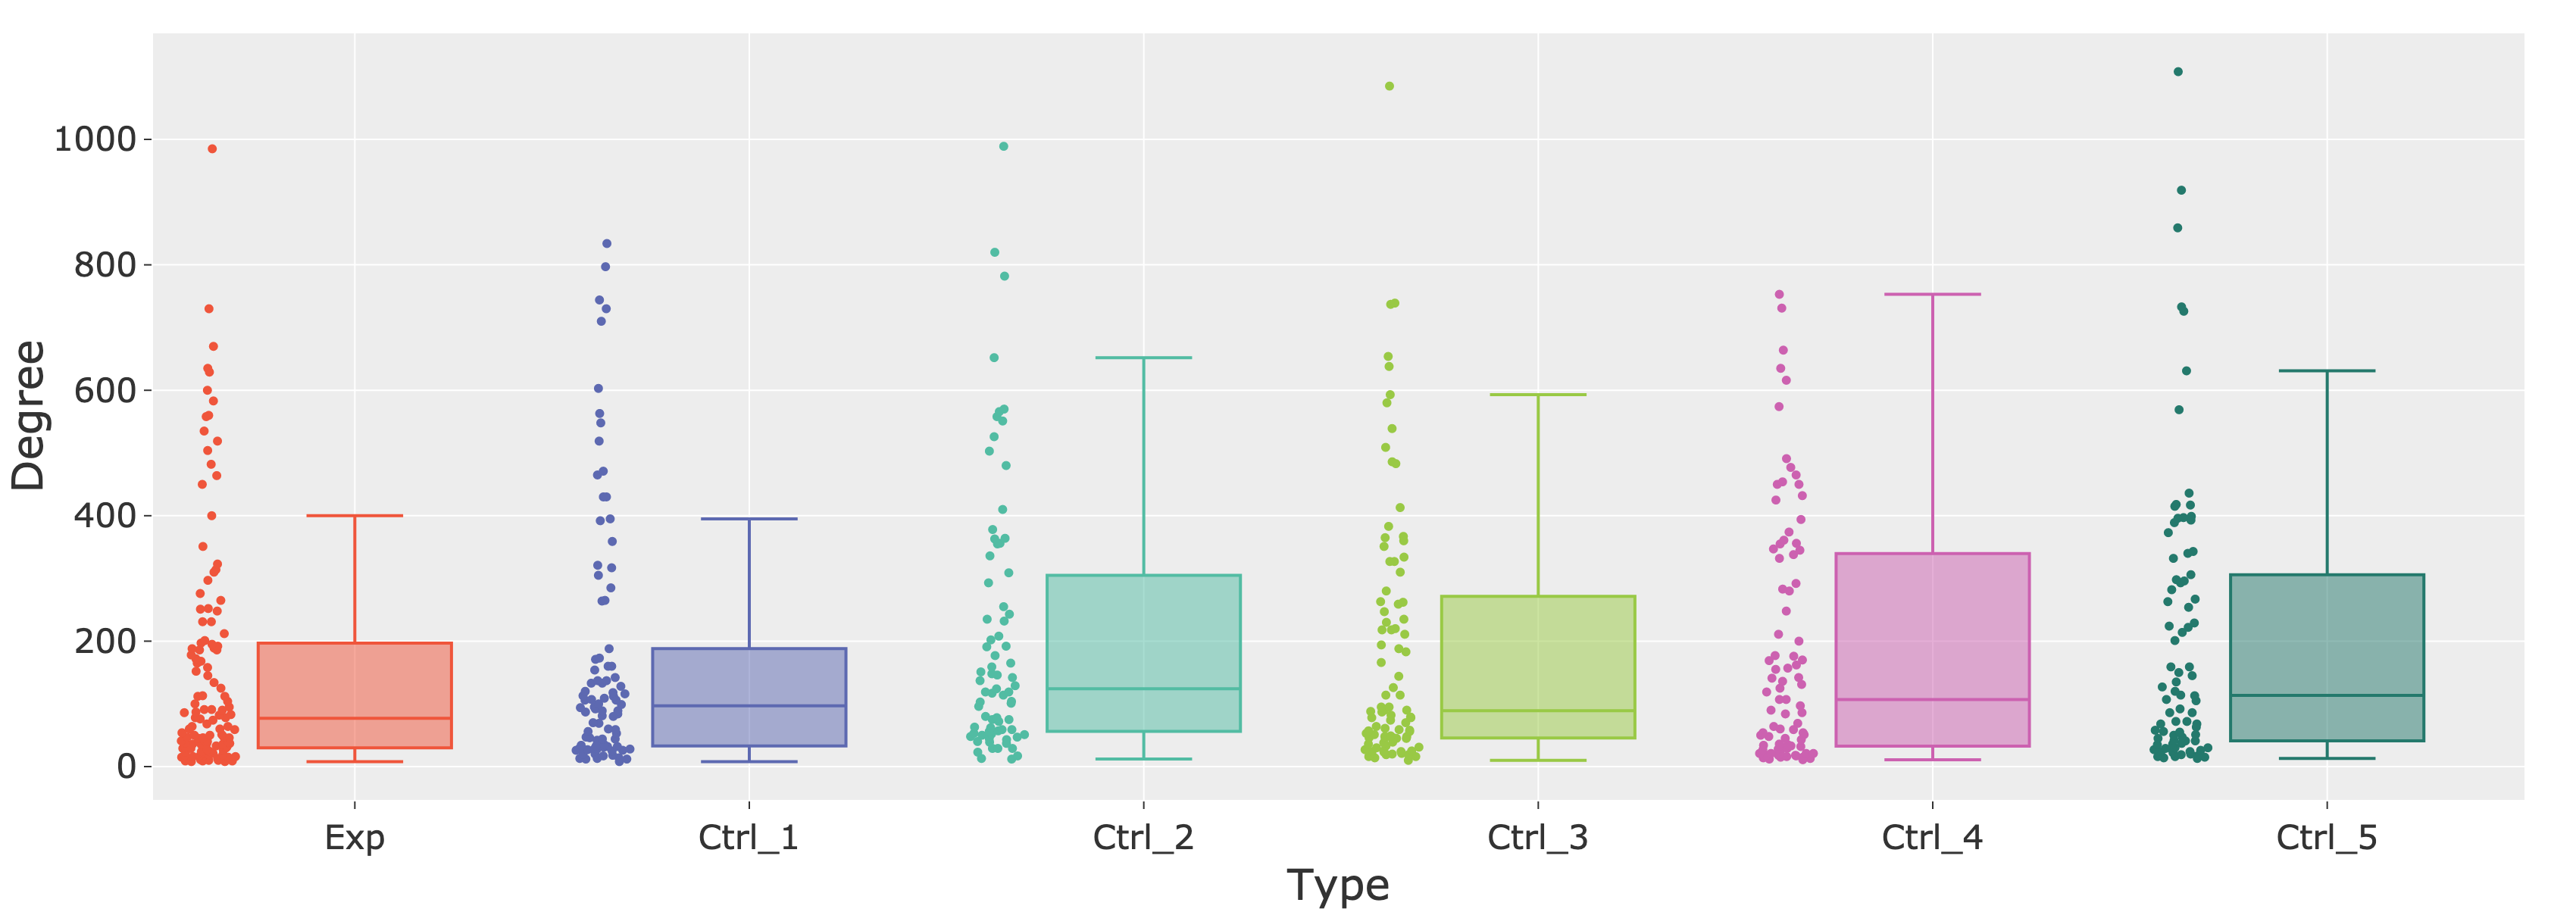
\includegraphics[width=1.0\textwidth,height=1.0\textheight,keepaspectratio]{Sections/Network_II/resources/reward/ctr_degree.png}
   \caption[The degree of highly connected genes across control networks]{Box plot showing the distribution of the highly connected genes across the five controls and the experiment. This shows that the mutation burden is essential for a gene to have a high degree. No significant difference was observed in the degree distributions (\acrshort{kw}: 8.668, p-value: 0.123).}
    \label{fig:N_II:ctrl_box}
\end{figure}


% Gene expression
\subsection{High degree: gene expression} \label{s:N_II:high_ge}

% Introduce the section
The previous sections showed that the 14 communities with the highest mean degree contain genes that need to meet several conditions to obtain that many connections. Biologically, gene expression is the proxy for their presence in the tissue, and it is the final (available) indicator of their importance in the MIBC, it is next used to understand genes' importance in the biological context.

% The 14 communities gene expression
The bar plot in \cref{fig:N_II:exp_molecular_highCon} shows the expression across the MIBC cohort of the 122 genes from the highly connected genes with the bar representing the standard deviation\footnote{This is a similar plot to \cref{fig:N_I:sel_tfs_var} used to refine the  98 TF from \cref{s:ap:sel_prun}.}. It shows that most of the genes have a TPM higher than 1, and 39/122 have a TPM less than 10. In addition, the error bars indicate which genes have a high standard deviation across the samples, an indicator of variability which can help isolating genes specific to subgroups. 



% Community 1
\textit{ELF3}, \textit{KLF5}, and \textit{CDH2} are part of community 1, which has the highest mean degree. The former is an early differentiation marker of urothelium \citep{Bock2014-zy}, while \textit{KLF5} has been associated with ABS-Ca differentiation earlier in the project \cref{tab:N_I:markers_diff} and in research from JBU \citet{Bock2014-zy}. \textit{CDH2} is part of the markers for the \acrfull{emt} signature, which is specific to the Luminal-Infiltrated subtype in TCGA cohort \citep{Robertson2017-mg}, see \cref{tab:lit:tcga_genes}.

% Community 2
Community 2 has the third largest mean degree and contains genes such as \textit{AHR}, \textit{CREBBP}, and \textit{NCOA1}. \textit{AHR} is overexpressed in Luminal tumours \citep{Shi2020-km} and associated with a poorer treatment response \citep{Ma2023-uu}. \textit{CREBBP} is involved in chromatin remodelling, and in the in situ experiments and bioinformatics analysis by \citep{Duex2018-qg}, it was found that targeting this gene has the potential to improve therapy. \textit{NCOA1} is also involved in chromatin remodelling, as noted in the \href{https://www.uniprot.org/uniprotkb/Q15788/entry#function}{Gene Card}.

% Community 3
\textit{LAMA3} and \textit{LAMA4} are part of the same gene family, and a genomic analysis study  \citep{Ma2024-xc} identified that these two genes are correlated with cell proliferation and migrations in bladder cancer. In a bioinformatics analysis focusing on cadmium exposure and its effect on bladder cancer, the authors in \citep{Zhang2023-ul} identified the overexpression of \textit{FN1} as a potential indicator of tumour purity and poorer survival prognosis. A relationship between \textit{FN1} and tumour impurity was also observed by \citep{Zhang2023-kv}.
The work of \citet{Guo2023-sf} studies the role of the collagen family, of which \textit{COL7A1} is part of, and it was found that these genes are associated with squamous subtypes. It is pointing out that \textit{COL7A1}, \textit{FN1}, and \textit{LAMA3} are all part of community 10, which has the second highest mean degree.


\begin{figure}[!t]    
    \centering
    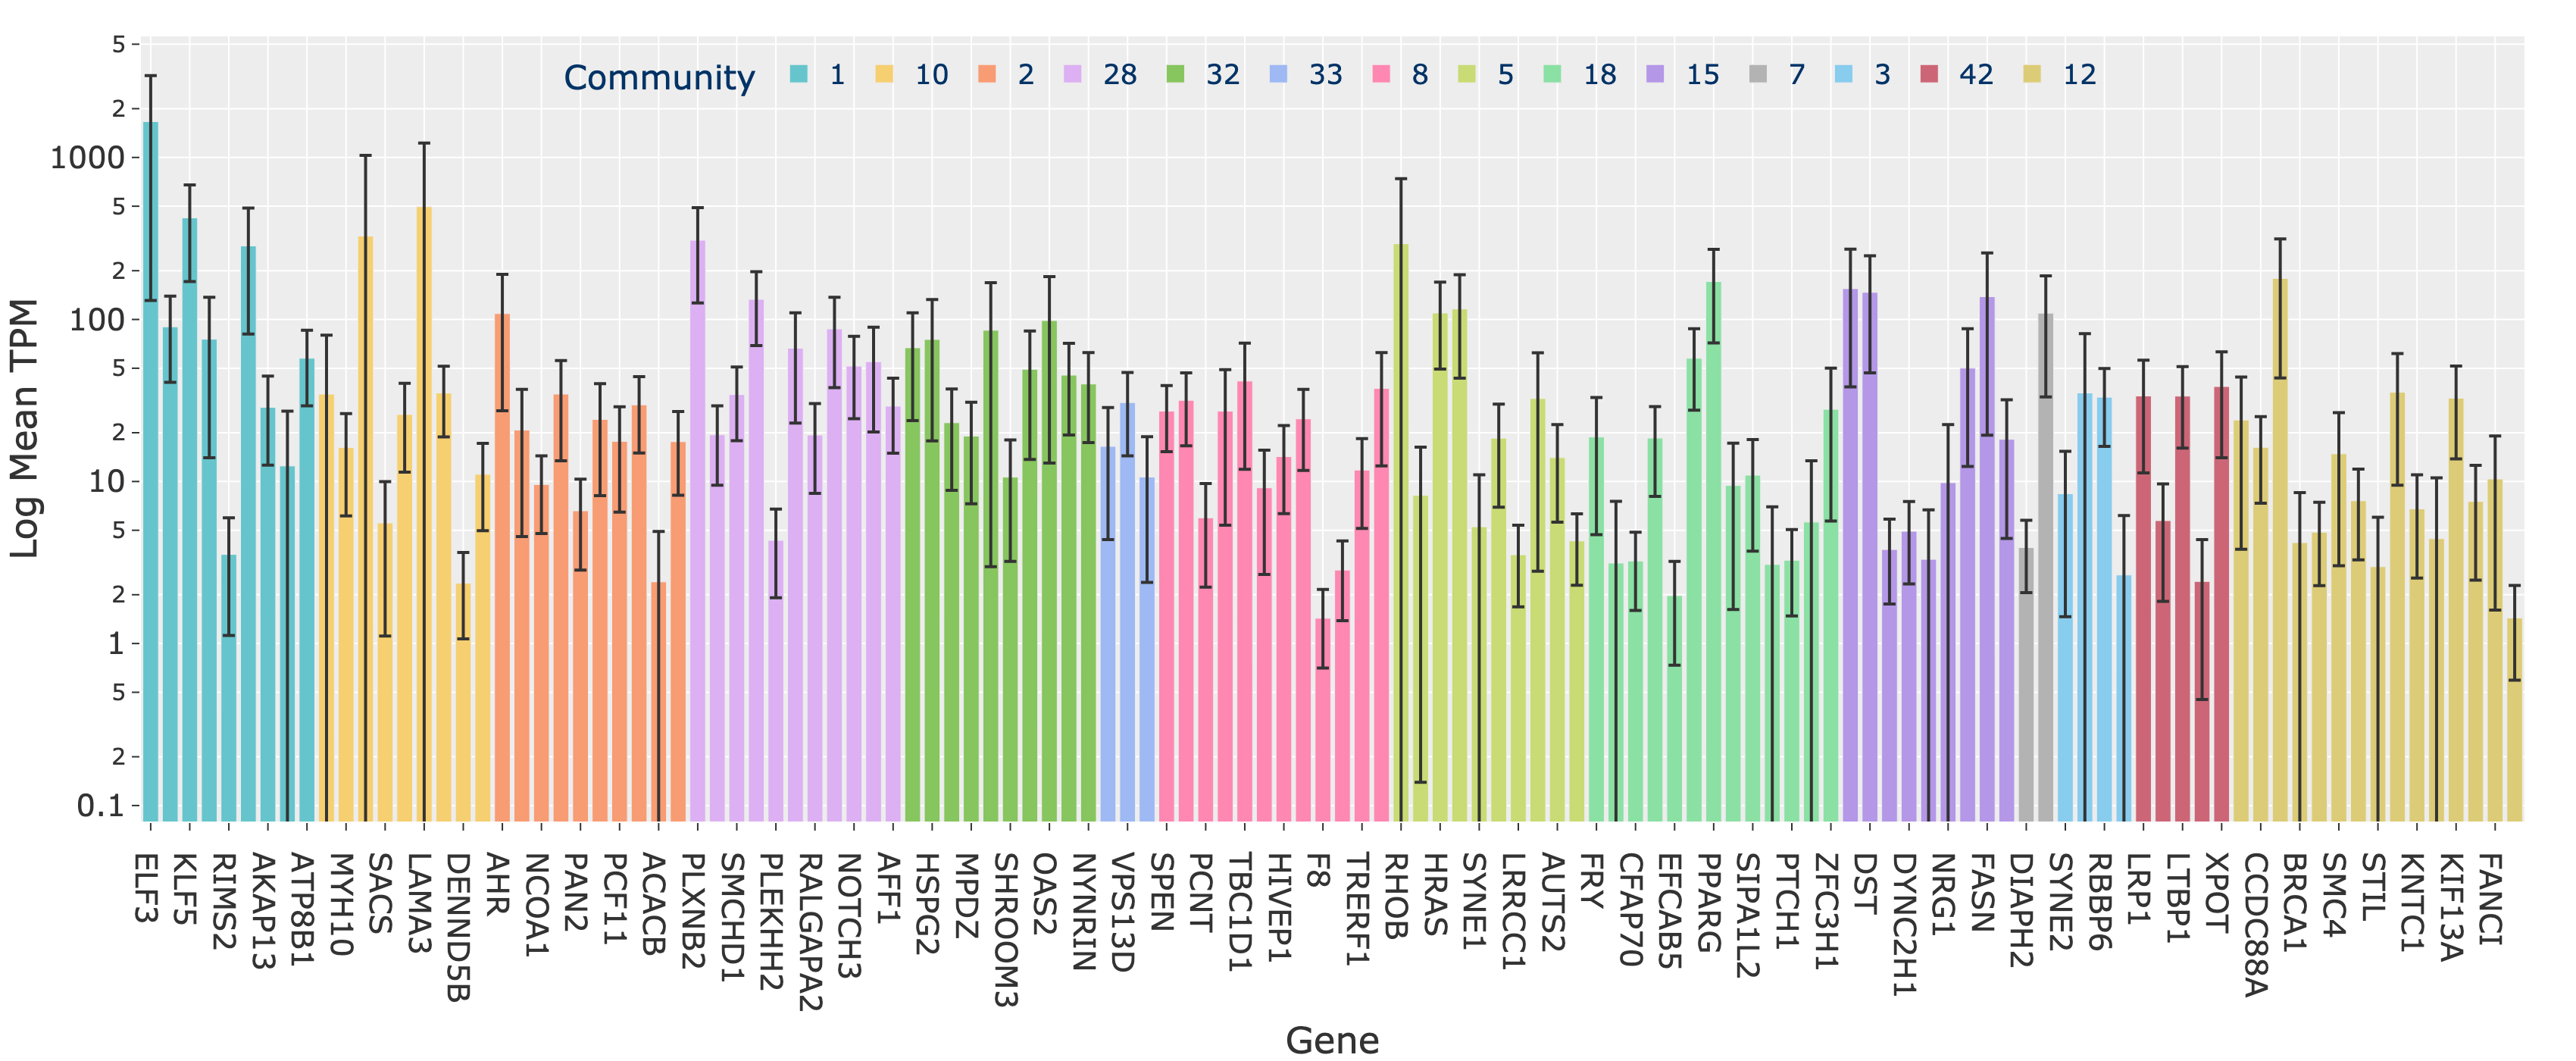
\includegraphics[width=1.0\textwidth,height=1.0\textheight,keepaspectratio]{Sections/Network_II/resources/reward/smallCom_Exp.png}
   \caption[Tumour median TPMs of highly connected genes]{Bar plot showing the tumour median expression on a log scale (Y) across the high connected genes (X). The bar colour represents the community membership and the error bar the standard deviation. Most of the highly connected genes have a TPM value larger than 1 and $\sim60\%$ have above 10. }
    \label{fig:N_II:exp_molecular_highCon}
\end{figure}


Exploring the three communities with the highest mean degree shows that the genes with a high number of connections have a biological function. Although the other blocks remain unexplored, there are many genes, such as \textit{FGFR3}, \textit{TP63}, and \textit{CDKN2A}, that are known to play a role in bladder cancer \citep{Robertson2017-mg,Kamoun2020-tj,Marzouka2018-ge,Choi2014-ed}, see tables with subtypes specific genes \cref{tab:lit:lund_genes,tab:lit:tcga_genes,tab:lit:consensus_genes}. This demonstrates the power of the network pipeline to isolate genes that have a functional role in bladder cancer, as studied in the literature, and to reveal new associations that have the potential to advance the understanding of bladder biology.

A cluster analysis on the MIBC cohort from TCGA was performed using either the tumour gene expression of the 122 highly connected genes or the MEVs from their corresponding communities, but the Basal/Luminal groups were not split into smaller groups. Due to this and the limited time available in a PhD, this cluster analysis was not covered more extensively in this thesis.



% MIBC subtyping
\subsection{MIBC subtyping}

% Introduce and motivate why we are choosing all the communities
So far, the work presented in this chapter has been focused on showing the data integration works and explaining that the 14 communities with a high mean degree are biologically functional and not a computational artefact. With this evidence that altering MEV and incorporating the mutation with the sigmoid reward function, the network approach created biologically relevant hubs which drastically altered network topology; all communities can now be applied to subtype the MIBC samples.

From the 45 communities in the reward network, the top 100 genes are selected using ModCon, and then the iMEV is applied (see \cref{s:N_II:iMEV}). On these values, a similar cluster analysis as in the earlier chapter is performed (see \cref{s:cs:methods}) and is covered in more depth in the Appendix \cref{s:ap:N_II:clustering analysis}. K-means with K=7 were chosen to stratify the MIBC, and the output is compared with the previous classification in \cref{fig:N_II:mibc_comp}.

% Basal groups
In \cref{fig:N_II:mibc_comp} cluster 1 (79 samples) contains the largest proportion of the Basal samples out of the Network II subtyping regardless of their \acrlong{ifn} response. Cluster 5 (31 samples) is also a Basal group which mainly consists of High and Low \acrshort{ifn} samples (CA+IFNG) as well as some Neuroendocrine (Ne) samples; the specific immune response of the cluster was supported by the DEA from \cref{fig:N_II:pi_basal_5}. Both groups (1 \& 5) have the lowest survival rate over 5 years, as seen in \cref{fig:N_II:survival_K_7}, with patients group 1 having a poorer prognosis than the other Basal group. Despite the Low IFNG and Ne samples, which are associated with a poorer prognosis, group 5 survival rate is in alignment with the previous work presented in this thesis, \cref{s:cs:basal_interp}, where the patient classified as higher \acrshort{ifn} have better survival chances.

% Luminal infiltrated groups
The largest group, 0 - 84 samples, contains some basal (TCGA/consensus) and LumInf samples by TCGA or a combination of Stroma-rich, LumNS, and Lump. Group 4 (56 samples) is also diverse, containing samples from LumInf-like groups similar to 0, but the remainder of the samples are classified as LumP by TCGA/Consensus. This may suggest two tendencies in the Luminal infiltrated samples, where the samples from 0 tend towards Basal phenotype while in 4 towards Luminal. The survival plot, \cref{fig:N_II:survival_K_7}, confirms this hypothesis by group 0 (yellow) having a worse prognosis than group 4.

% Luminal Papillary
Group 3 (67) is mainly composed of Luminal Papillary (LumP) samples (TCGA, consensus) but also contains samples from other luminal groups such as Luminal Unstable (LumU) or LumNS (Luminal Non-specified) as well as a few Basal. Groups 6 (18) and 2 (69) are both comprised of mainly LumP groups with a few minor exceptions. The Luminal tendencies are also confirmed by the favourable survival rates seen in \cref{fig:N_II:survival_K_7}.

\begin{figure}[!htb]
    \centering
    \begin{subfigure}[!t]{1.0\textwidth}
        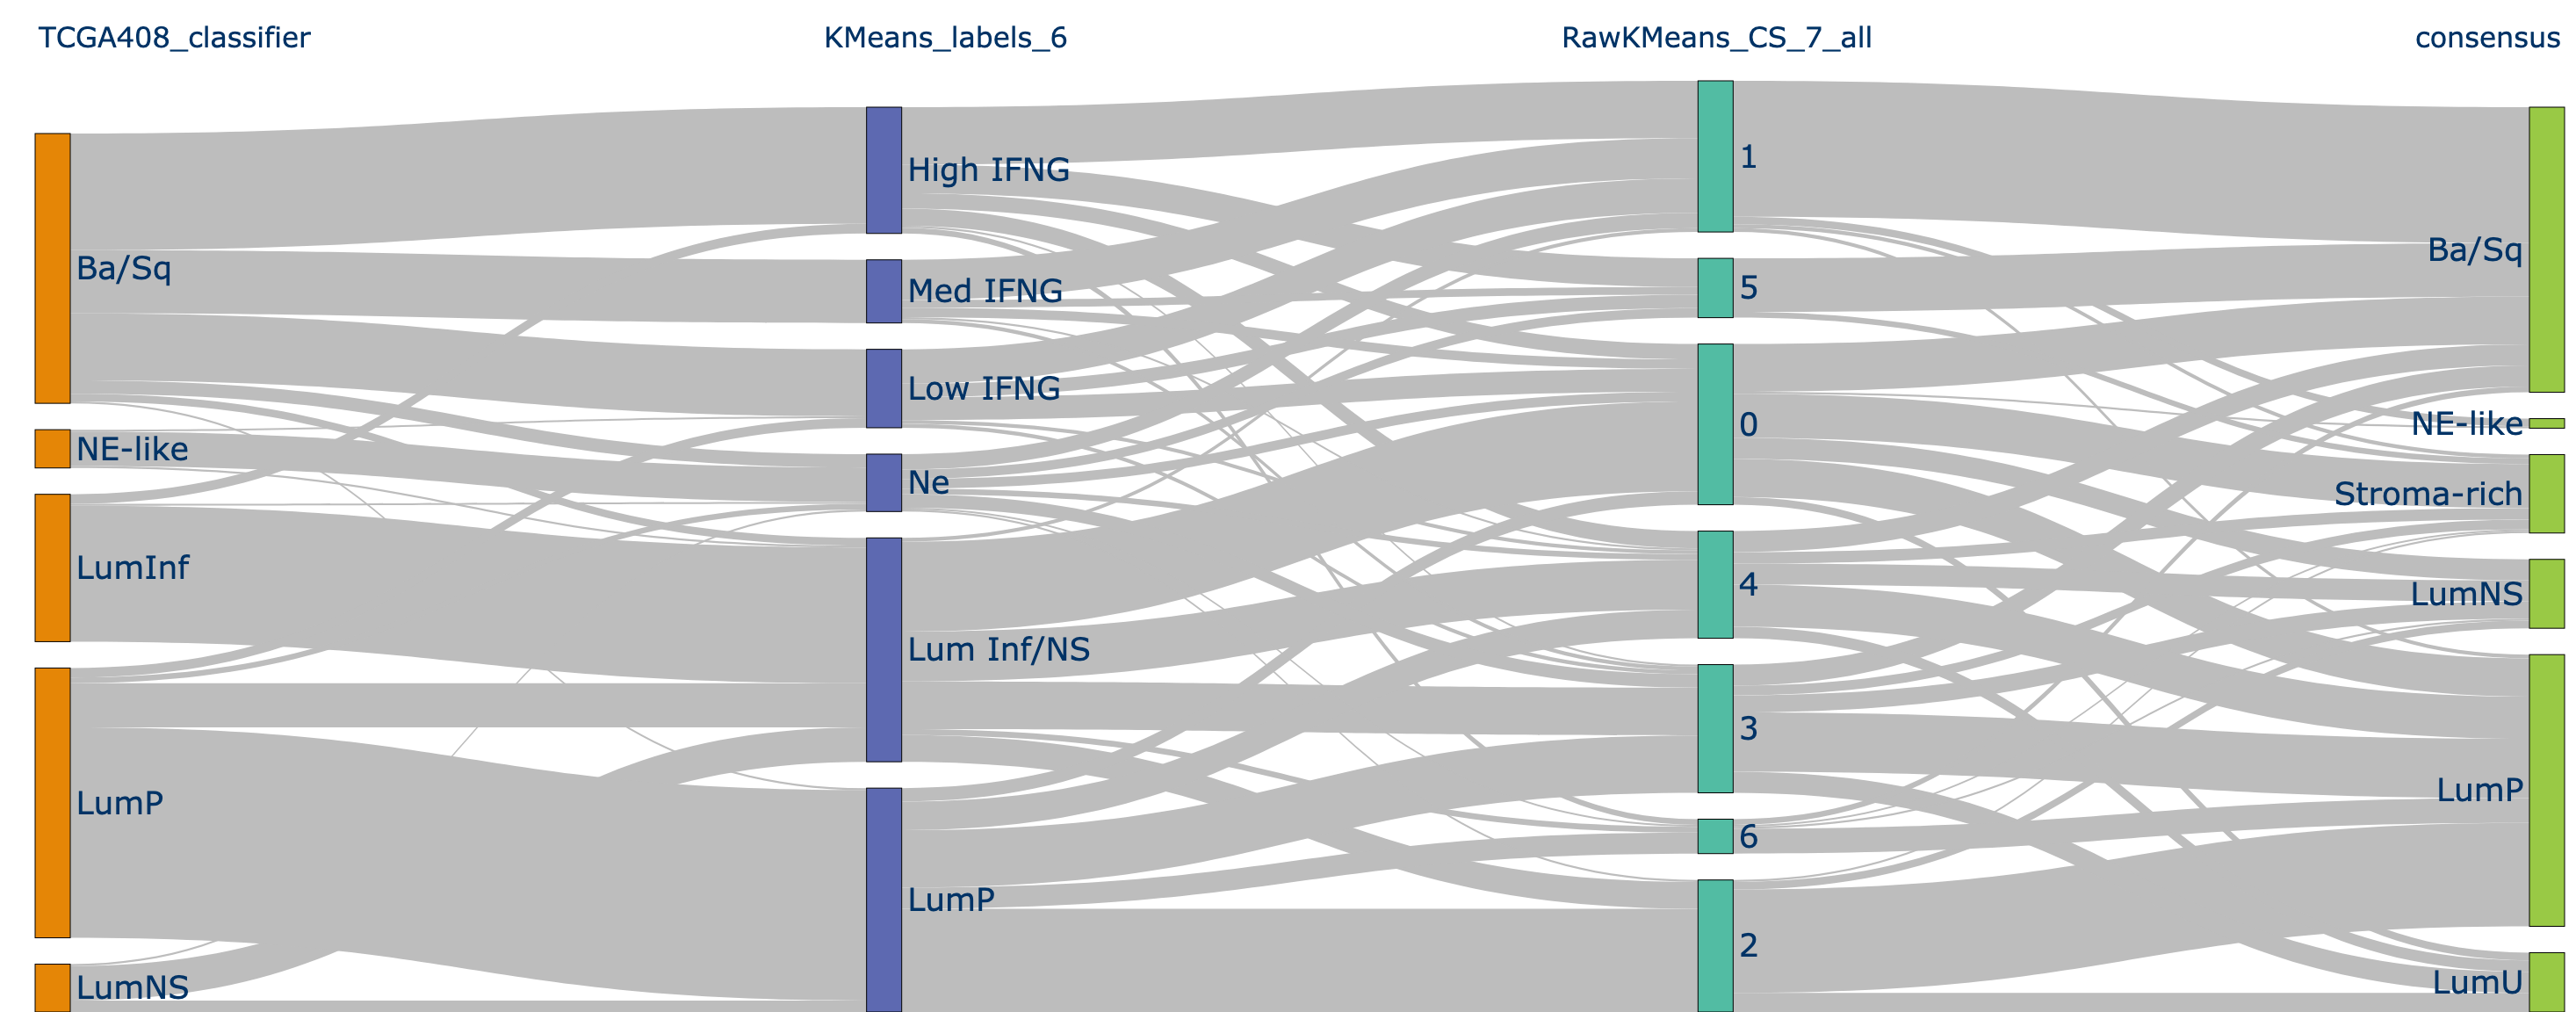
\includegraphics[width=1.0\textwidth,height=1.0\textheight,keepaspectratio]{Sections/Network_II/resources/reward/cluster_comp_final.png}
        \caption{Comparison of the MIBC subtype derived using the second version of the network approach introduced in \cref{s:N_II:rwd}, where the MEVs are grouped with K-means K=7. These subgroups are compared with the classifications from TCGA \citep{Robertson2017-mg}, the consensus \citep{Kamoun2020-tj}, and the previous subtypes derived using the cluster analysis from \cref{s:clustering_analysis}. The black font text in front of the subtypes from K-means represents the community seize.}
        \label{fig:N_II:mibc_comp}
    \end{subfigure}
    \begin{subfigure}[!t]{1.0\textwidth}
        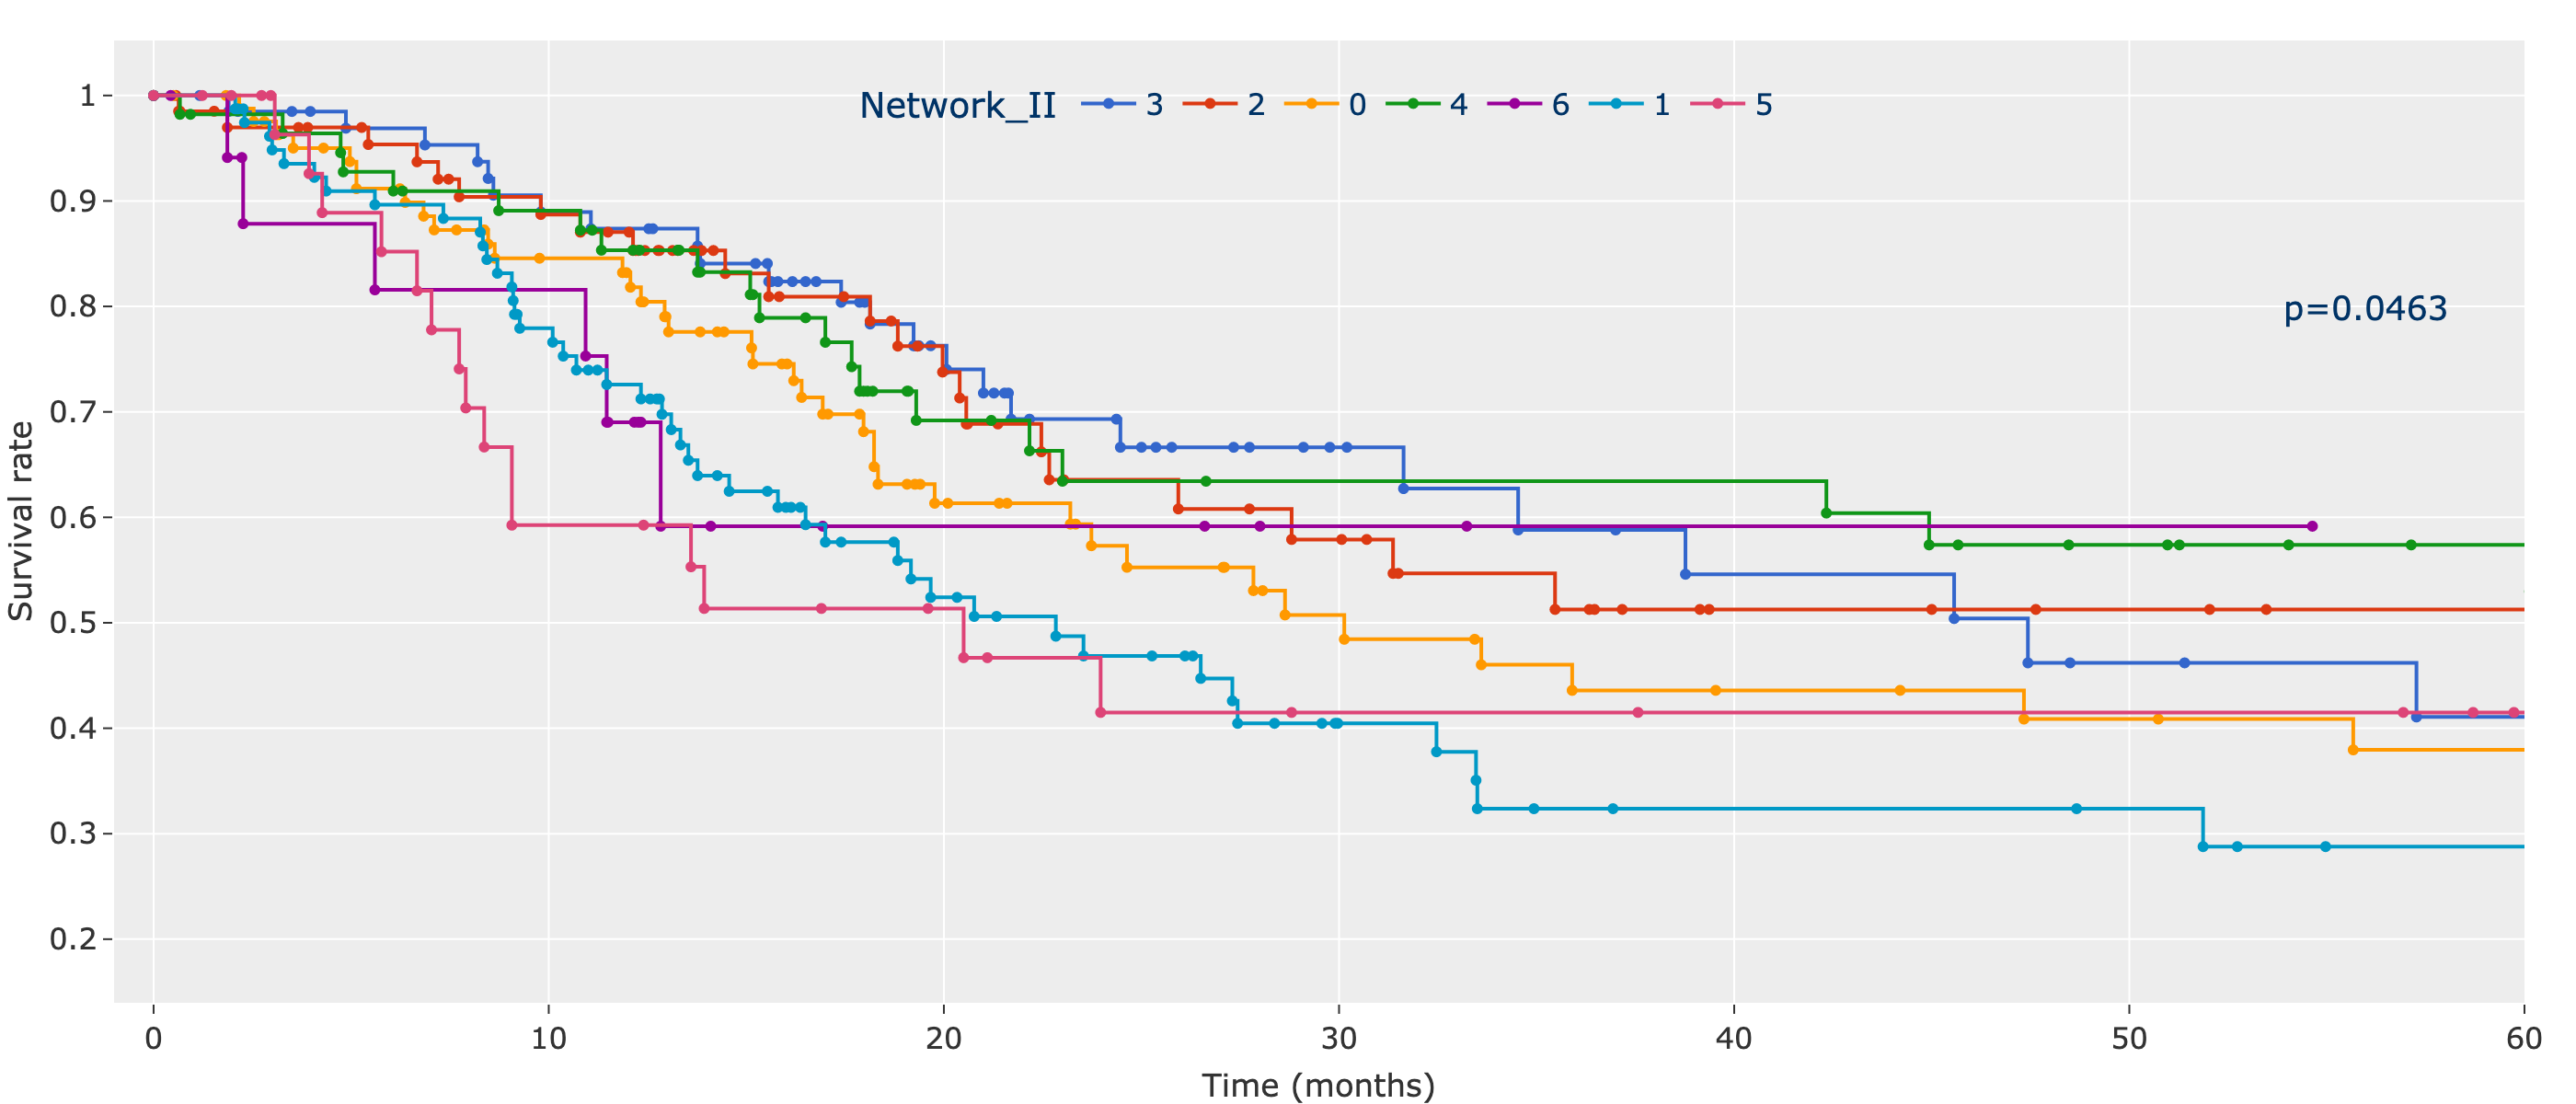
\includegraphics[width=1.0\textwidth,height=1.0\textheight,keepaspectratio]{Sections/Network_II/resources/reward/cluster_analysis/survival_K_7.png}
        \caption[Overview of the MIBC subgroups derived from the non-tumour reward network]{Kaplan-Meier survival analysis of the 7 groups derived using the MEV scores and K-means (see \ref{s:ap:N_II:clustering analysis} for discussion). The plot shows the two trends in survival between the three Basal and two Luminal groups. A similar figure but with K=5 is can be seen in \cref{fig:ap:survival_K_5}. }
        \label{fig:N_II:survival_K_7}
    \end{subfigure} 
    \caption[Refined rewad network: MIBC overview]{Overview of the MIBC splits using the reward network and the pipeline proposed in this chapter}
\end{figure}


% DEA
\subsection{Differential Expression Analysis} \label{s:N_II:dea_rwd}

% Basal
\subsubsection*{Basal} \label{s:N_II:basal}

% Introduce Basal 5
The Basal groups 1 and 5 have the poorest survival prognosis and are both explored in the Pi plot from \cref{fig:N_II:pi_basal_5}. While the focus of the Pi-plot is on Basal 5, it can be seen that groups 0 and 5 do not share many common genes, and each has its subset of genes specific to its group when compared to Basal 5. This is unexpected as both groups consist of previously clustered samples as either Luminal Infiltrated or High IFNG.

% Comment on the Pi-plot
The 'Ref point' in the bottom left represents the X and Y minimum values, denoting the most 'Basal 5' specific point. The top 10 closest points to the referential point are displayed, and it can be noticed that most of the genes are Ensembl genes, denoting the unexplored nature of the genes found. However, there are some genes, such as \textit{MT2A}, \textit{MT1X}, and \textit{KRT6B}, which are specific to Basal 5 in comparison with Basal 1. \textit{MT2A} was found in \textit{in vitro} experiments by to be a tumour suppressor, as its knockdown increased cell invasion and growth \citep{Sung2022-tm}. \textit{MT1X}, along with other metallothioneins (including \textit{MT2A}), was reviewed by \citep{Si2018-ep} and found to have the potential to be a biomarker for cancer diagnosis. \textit{KRT6B} is part of the Keratinization signature specific to the Ba/Sq group; see Lund markers in \cref{tab:lit:lund_genes}.

% Squamous
Less clear in the Pi-plot is that many markers for upregulated Squamous Cell Carcinoma (SCC) from \citep{Hurst2022-sp} are present on the negative side of the Y-axis, being specific to the Basal group 5; \textit{HMGA2} is one such marker. On the positive side of the vertical axis are the downregulated SCC markers shown in dark yellow, as well as other genes such as \textit{UPK} and \textit{ELF3}, which are specific to luminal groups; see Lund table \cref{tab:lit:lund_genes}.

\begin{sidewaysfigure}
    \centering
    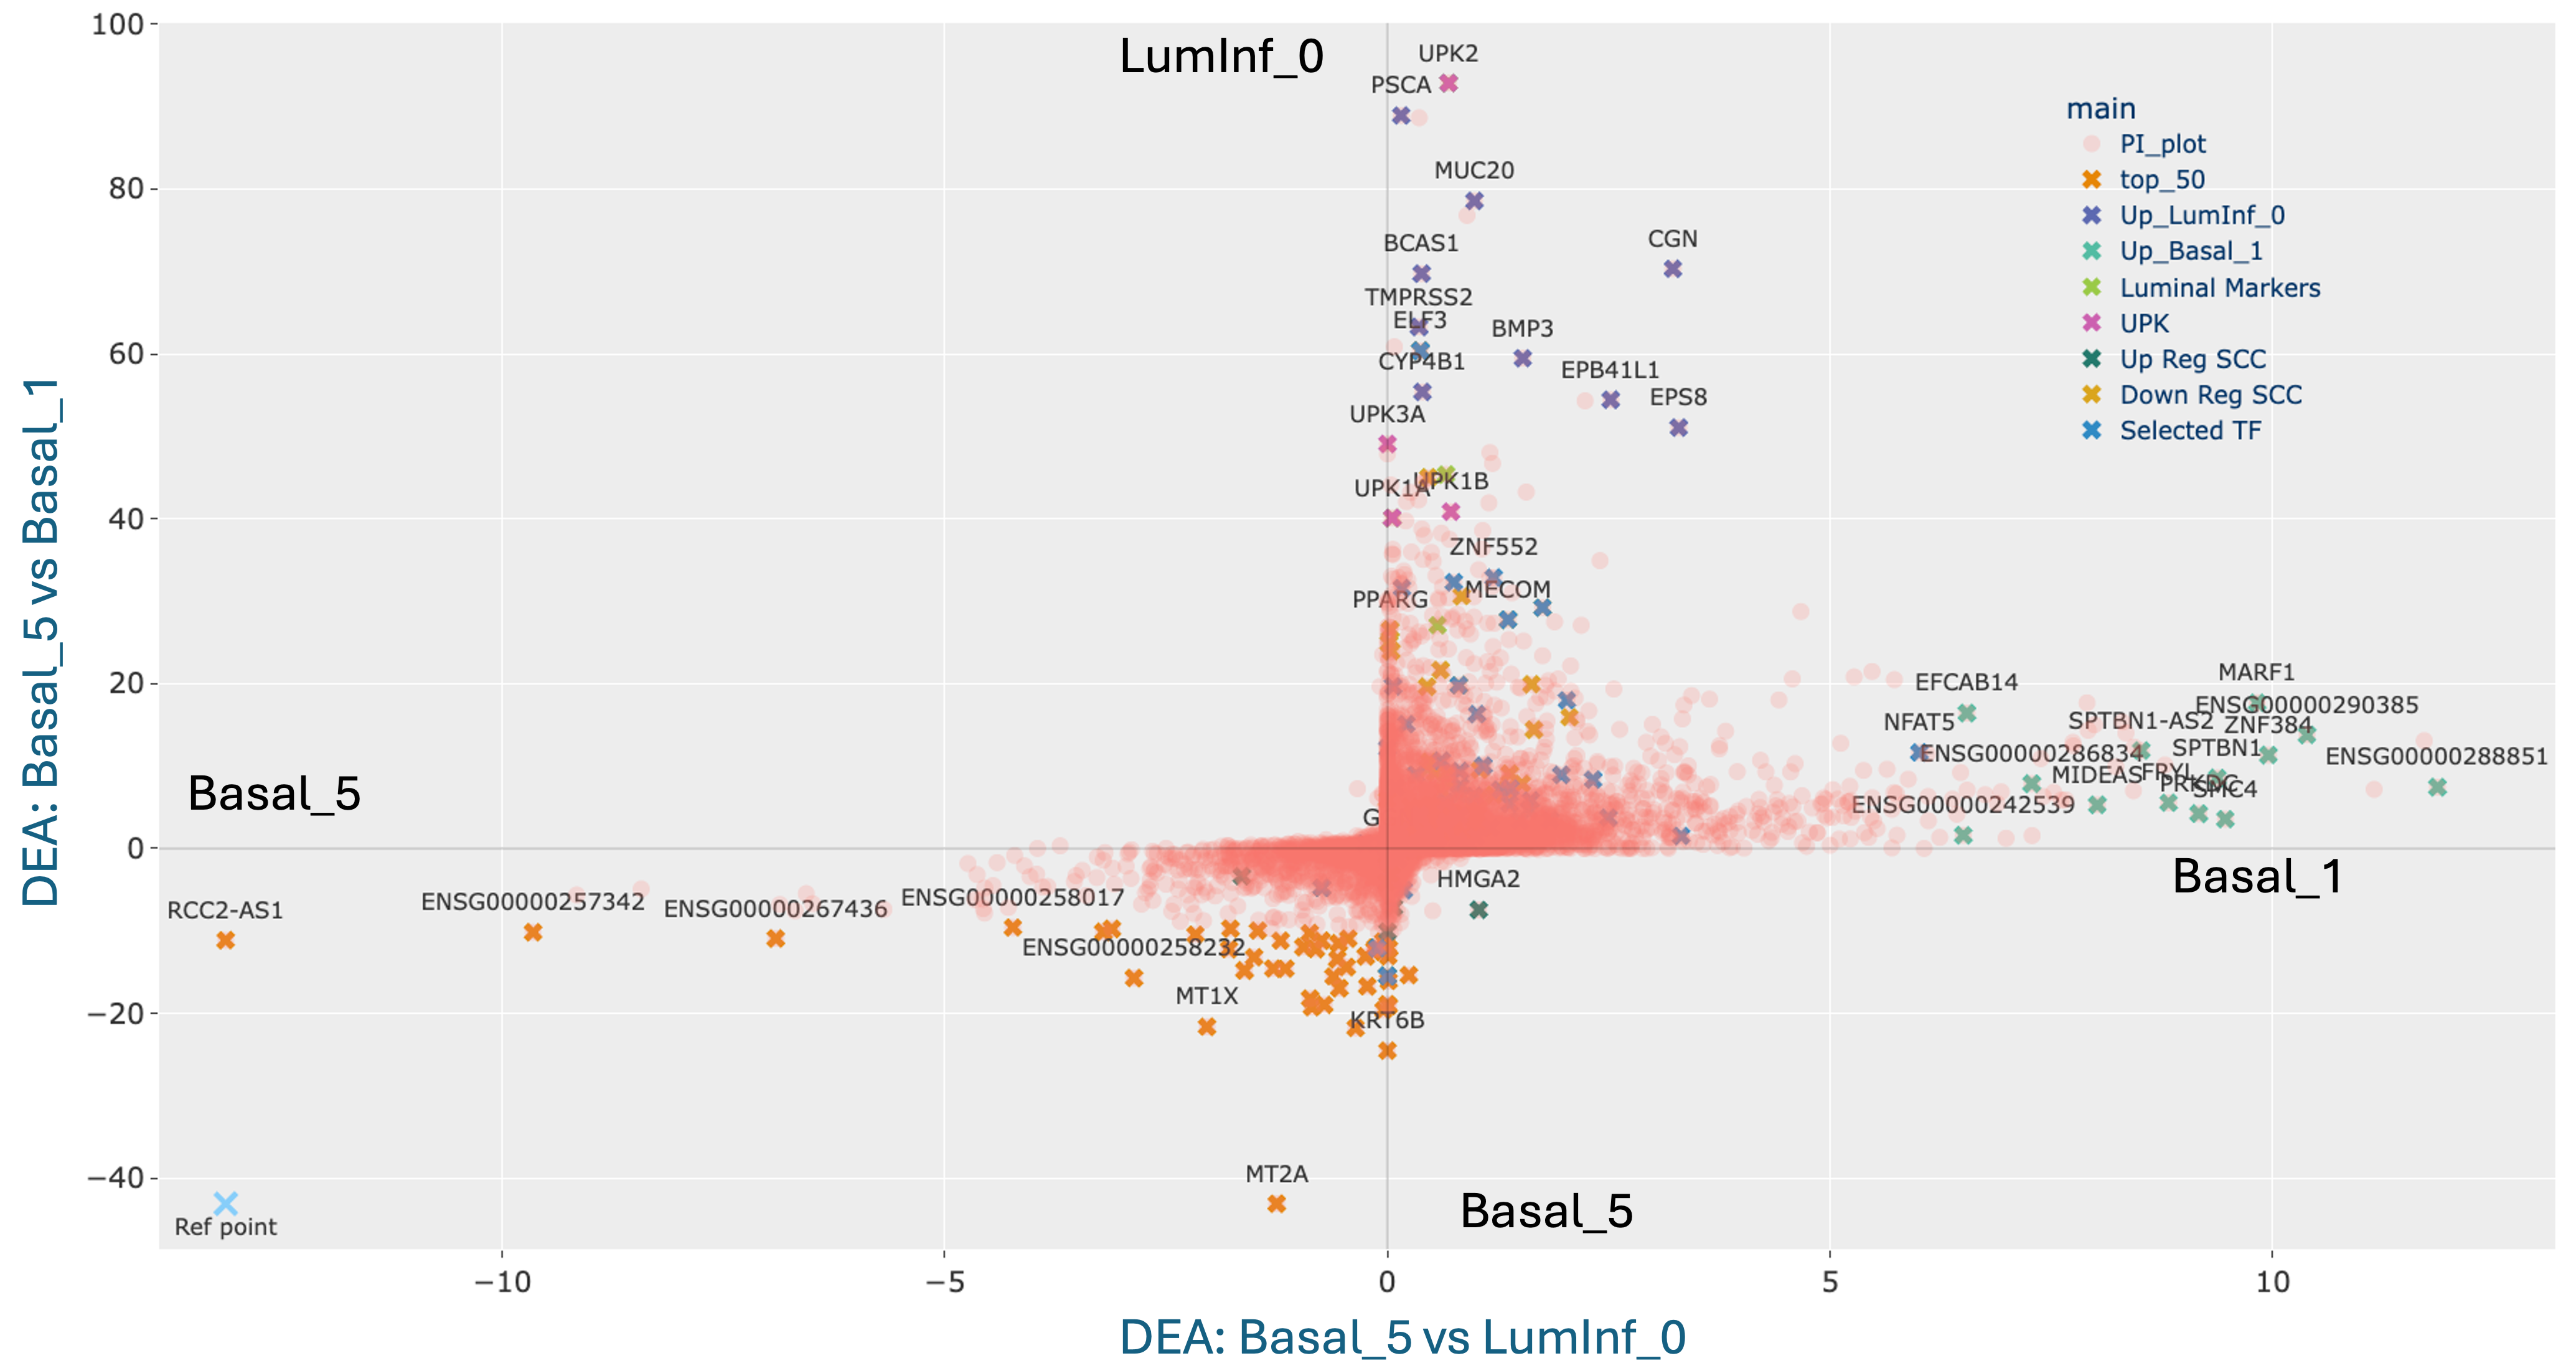
\includegraphics[width=1.0\textwidth,height=1.0\textheight,keepaspectratio]{Sections/Network_II/resources/reward/PI_Basal_5.png}
    \caption[Pi plot highlighting the properties for Basal 5]{The Pi plot with the \acrshort{dea} between Basal 5 and LumInf 0 (X-axis) and Basal 1 (Y-axis); following the methods from \cref{s:lit:pi}. The points in distinct colours representing different known markers, such as Luminal Markers, UPK, Up and Downs Regulated genes in \gls{SCC}, the 98 TF found in previous sections \cref{s:N_I:sel_tfs}, as well as some of the highly significantly expressed genes in the two comparisons (Up\_LumInf\_0 and Up\_Basal\_1). The points in the third quadrant represent the genes that are most specific to group 5, while the first quadrant contains the genes specific to both clusters 0 and 1.}
    \label{fig:N_II:pi_basal_5}
\end{sidewaysfigure}


% Basal 1
On the positive side of the X-axis are the markers specific to the Basal 1 group compared to Basal 5. Only four unnamed Ensembl genes are shown for visualisation, but more are expressed in the DEA. There is also a \acrlong{tf}, \textit{NFAT5}, that was previously identified in the selective edge pruning work, \cref{s:N_I:sel_pruning}. It can also be noticed that \textit{SPTNB1} and its antisense \textit{SPTNB1-AS2} are present. In a proteogenomic study, \citep{Fanayan2013-uj} focused on colon cancer and found that these genes are potential tumour markers.

% Conclusion
The pi-plot in \cref{fig:N_II:pi_basal_5} affirms the 'Basalness' of groups 5 and 1, as well as the luminal properties of cluster 0. The analysis also shows that many significantly expressed genes between groups are \acrlong{lncRNA}, denoting uncharted territory and indicating the potential for new biological discoveries.



% Luminal
\subsubsection*{Luminal 6} \label{s:N_II:lum_6}

Group 6 from \cref{fig:N_II:mibc_comp} is one of the smallest luminal groups found in this project, which also has a good survival prognosis \cref{fig:N_II:survival_K_7}. The first quadrant from \cref{fig:N_II:pi_lum_6}  represents the points that are specific to both Lum 3 and Lum 2, while the third quadrant contains all the genes that are specific to cluster 6. 

% Quadrant 3
The three studied groups contain samples that were previously classified as luminal. The goal of the pi-plot is to highlight any particular molecular properties of Lum 6 over the other luminal subtypes, which is clearly shown by the genes displayed in the third quadrant. From the shape of the scatter plot, it can be seen that there are only a few genes close to either the X or Y-axis, indicating that Lum 6 does not share many genes with the other two groups, especially with group 2, which consists solely of LumP samples (see Sankey \cref{fig:N_II:mibc_comp}). Most of the values specific to group 6 are unnamed Ensembl genes, which indicates the novelty of this finding. Concurrently, this makes it challenging to characterise the subtype.

% Quadrant 1
In the diagonally opposite quadrant are the genes that are specific to the other two luminal groups, 2 and 3. There are several luminal markers present, such as PI3K Pathways, genes involved in maintaining transitional phenotype \citep{Hurst2022-sp}, and the luminal markers from TCGA \cref{tab:lit:tcga_genes}. Most of the genes specific to the top right do not have a determined role in bladder cancer, and there are several Ensembl genes (only a few are shown for visualisation purposes). However, there are a few exceptions, such as \textit{HLTF} and \textit{SETD2}, which have known roles in cancer. \textit{HLTF} was studied by \citep{Dhont2016-vf}, who found that when the gene is silenced, it leads to more mutations in the genome, is present in the early stages of cancer, and is correlated with poorer prognosis. Both Lum 3 and Lum 2 have poorer survival rates than Lum 6, which is different from what the study suggests. In a pan-cancer analysis, the authors in \citep{Lu2021-jt} found that \textit{SETD2} mutation is correlated with a higher mutation burden and immune response across the cancer cohorts in TCGA and therefore with better survival.

% Conclusion
The analysis shows that Group 6 is different from the other groups by exhibiting strong differentially expressed markers in the DEA comparison with both Lum 2 and Lum 3. Unnamed genes were even more present than in the analysis of the basal groups (1, 5) from the previous sections. This indicates that the group has novel biological characteristics that are yet to be discovered.


\begin{sidewaysfigure}  
    \centering
    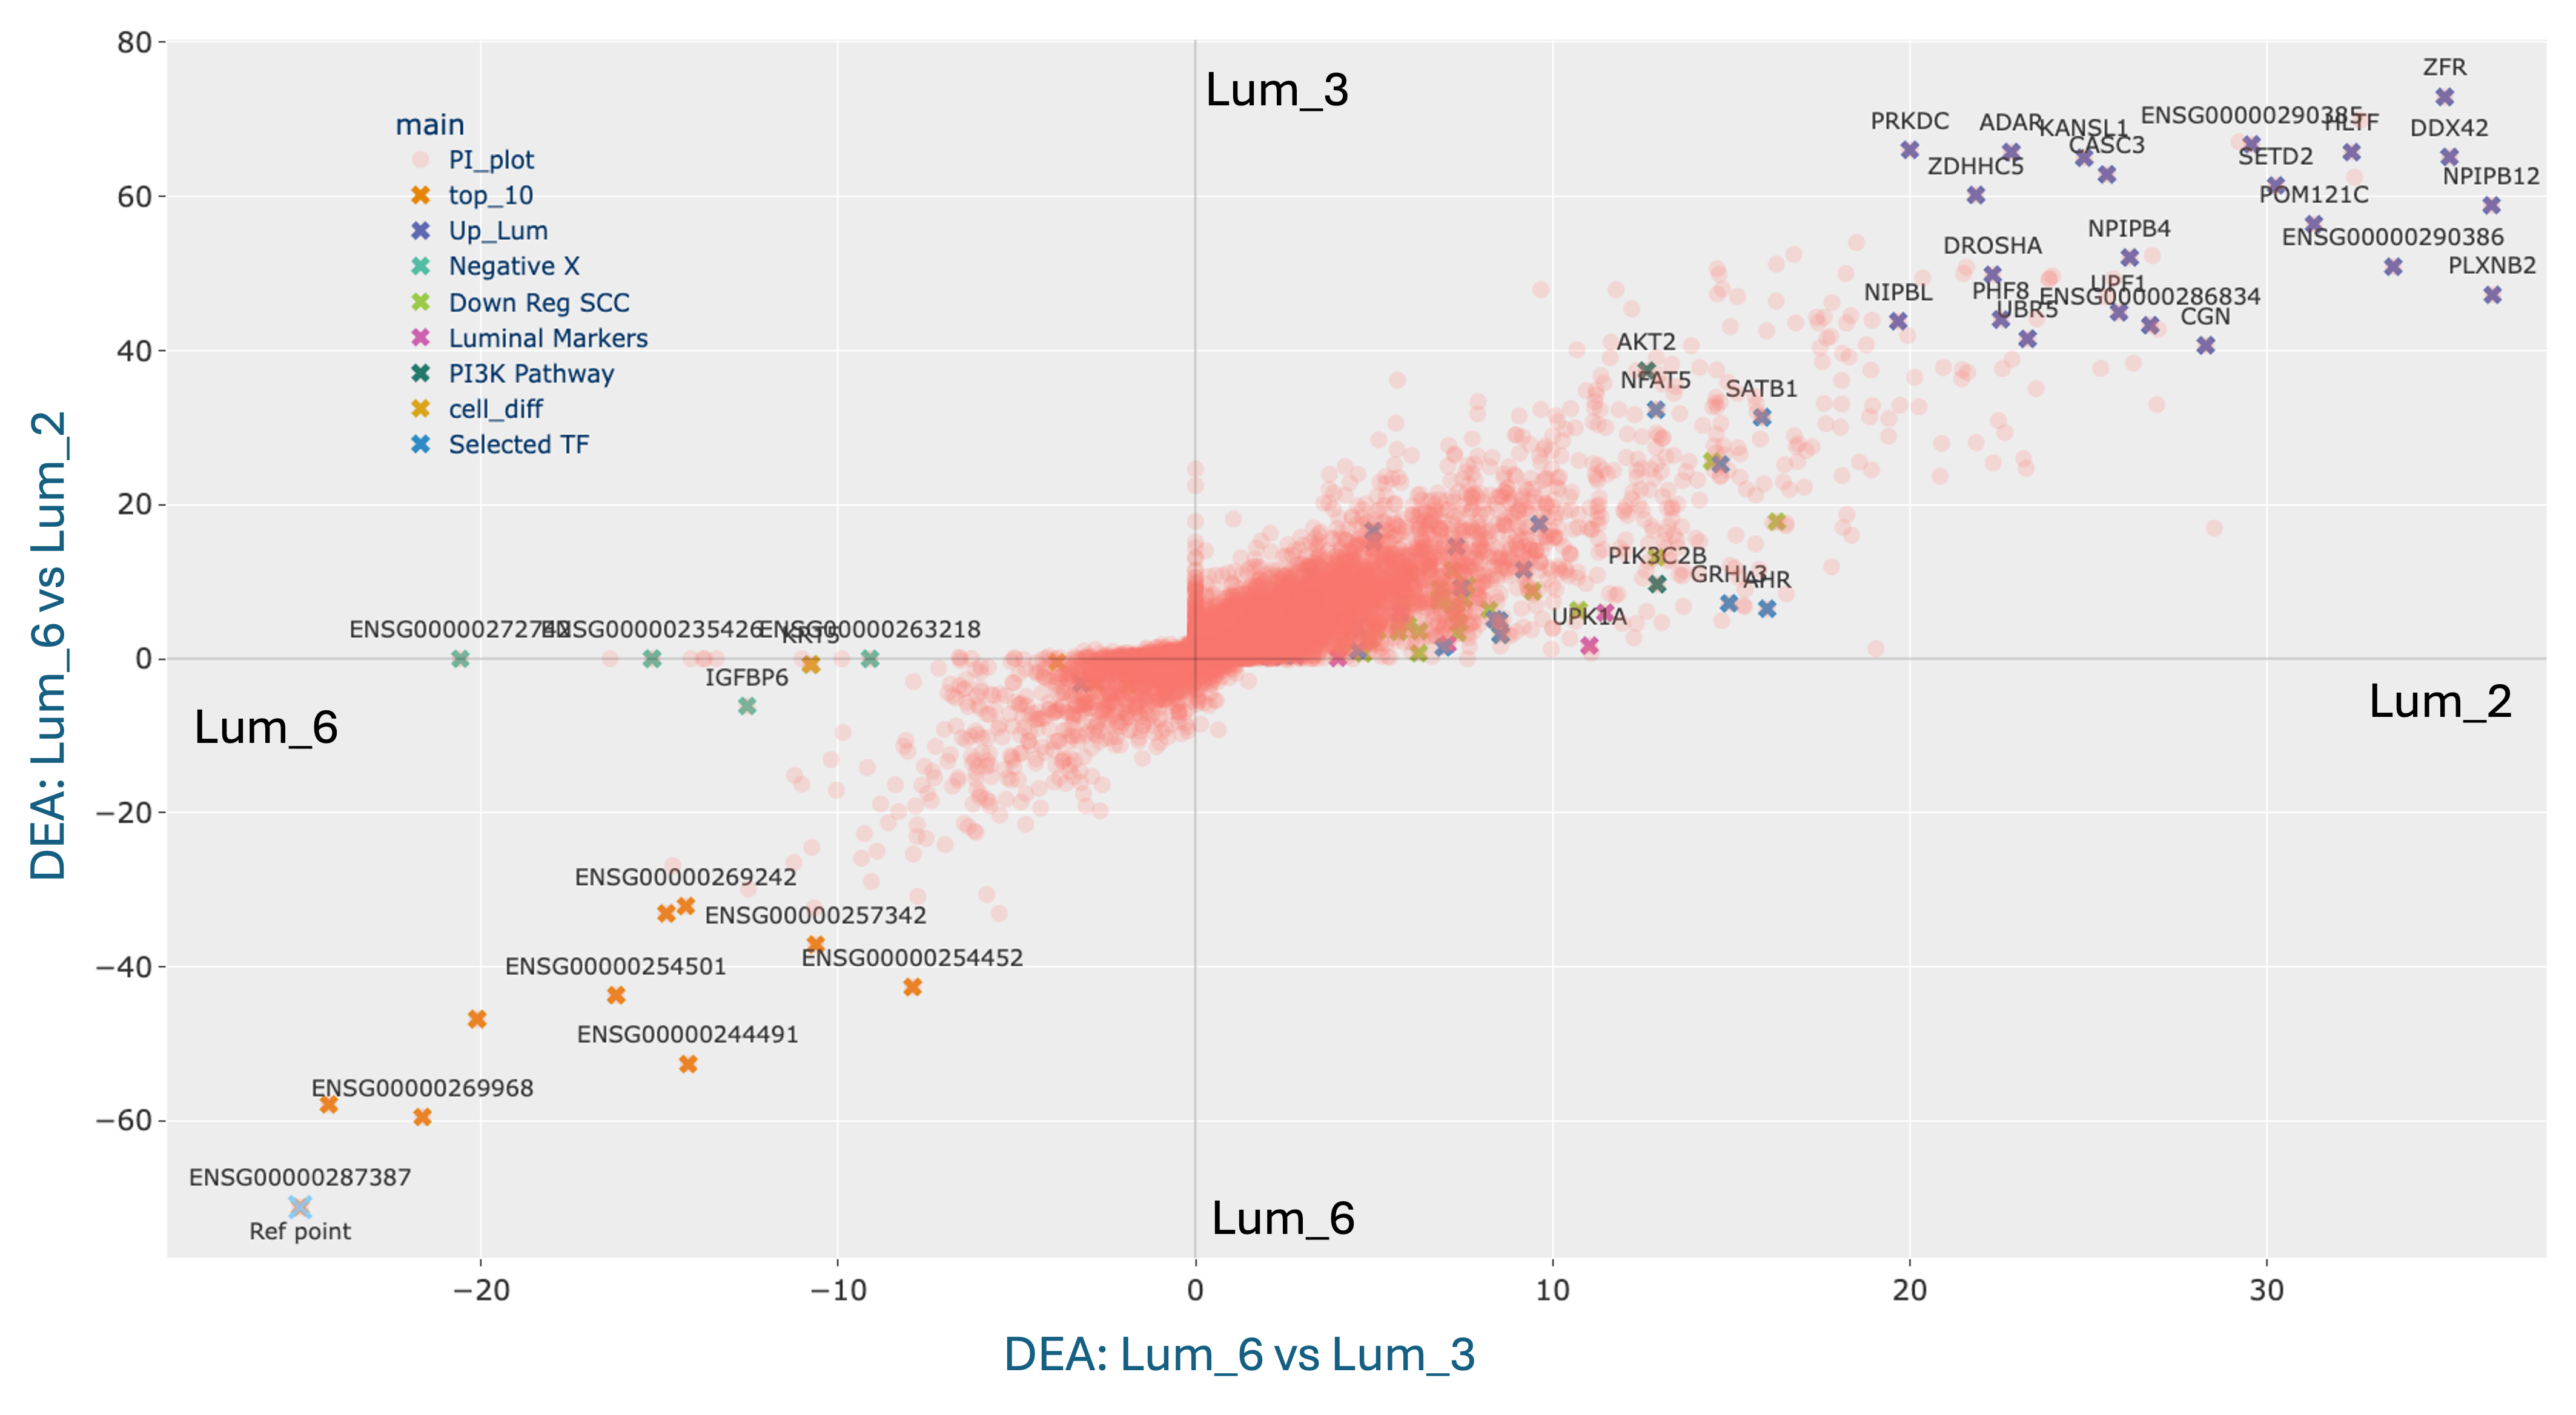
\includegraphics[width=1.0\textwidth,height=1.0\textheight,keepaspectratio]{Sections/Network_II/resources/reward/PI_Lum_6.png}
    \caption[Pi plot highlighting the properties for Lum 6]{The Pi plot with the \acrfull{dea} between Lum 6 and Lum 3 (X-axis) and Lum 2 (Y-axis); following the methods from \cref{s:lit:pi}. The points in distinct colours representing different known markers, such as Luminal Markers, UPK, Up and Downs Regulated genes in \acrlong{scc}, the 98 TF found in previous sections \cref{s:N_I:sel_tfs}, as well as some of the highly significantly expressed genes in the two comparisons the two comparisons (Up\_Lum) and the negative values on the X-axis (Negative X). The third quadrant highlights the genes specific to the Basal 6 group, while the first quadrant contains the genes more common to the other two groups. The analysis shows that there are many \acrshort{lncRNA} genes specific to the Luminal 6 groups.}
    \label{fig:N_II:pi_lum_6}
\end{sidewaysfigure}


\subsection{Summary}


% Highly connected communities
The work on the reward network shows that the new weight modifier successfully integrates the mutation burden into the non-tumour dataset. The approach identifies 14 communities with genes that meet the following conditions: 1) have a high mutation burden ($>$10), 2) are co-expressed with several other genes, and 3) the co-expressed genes have a strong correlation. There are 122 genes across the blocks, characterised by having a high number of connections. The small number of nodes in a community illustrates the power of the \acrlong{hsbm}, which is able to group even two genes (community 7) out of the 5000 genes. This indicates that the community detection algorithm would be able to accommodate a larger dataset.

% New MIBC subtypes
The reward network was then used to stratify the MIBC cohort from TCGA, revealing different subgroups compared to the work in the first chapter and other classifications. The analysis shows the two trends of the major MIBC subgroups: Basal (1, 5) and Luminal (2,6,3). In addition, there are the samples with a high infiltration 0 and 4, each with a tendency towards the Basal/Luminal types. 


% Focus on the 2 interesting groups
Basal 5 showed poor survival rate and exhibited some squamous markers, while Luminal 6 shows different molecular properties when compared with the other Luminal groups. In both cases, the markers defining these groups (i.e. significantly expressed) are mainly comprised of poorly described Ensembl genes. This suggests the opportunity to discover new biological insights.





